\documentclass[11pt,a4paper]{article}
\usepackage[french]{babel}
\usepackage[utf8]{inputenc}
\usepackage[T1]{fontenc}
\usepackage[cm]{fullpage}
\usepackage{graphicx}
\usepackage{listings}
\usepackage{epsfig}
\usepackage{enumitem}
\usepackage{xcolor}
\usepackage{color}
\usepackage{bbding}
\usepackage{array}
\usepackage{pdfpages}
\usepackage{tocloft}
\usepackage[french,frenchkw,boxed,ruled,lined]{algorithm2e}
\SetKw{KwDe}{de}
\SetKw{KwOu}{ou}
\SetKw{KwEt}{et}
\SetKw{Kwrenv}{renvoyer}
\SetKwInput{Variables}{Variables}
\SetKwInput{Variable}{Variable}
\usepackage{comment}

\definecolor{codegreen}{rgb}{0,0.6,0}
\definecolor{codegray}{rgb}{0.5,0.5,0.5}
\definecolor{codepurple}{rgb}{0.58,0,0.82}
\definecolor{backcolour}{rgb}{0.95,0.95,0.92}

\lstdefinestyle{mystyle}{
    backgroundcolor=\color{backcolour},   
    commentstyle=\color{codegreen},
    keywordstyle=\color{magenta},
    numberstyle=\tiny\color{codegray},
    stringstyle=\color{codepurple},
    basicstyle=\footnotesize,
    breakatwhitespace=false,         
    breaklines=true,                 
    captionpos=b,                    
    keepspaces=true,                 
    numbers=left,                    
    numbersep=5pt,                  
    showspaces=false,                
    showstringspaces=false,
    showtabs=false,                  
    tabsize=2,
    frame=single,
}
\lstdefinestyle{mystyle1}{
    commentstyle=\color{codegreen},
    keywordstyle=\color{blue},
    morekeywords={Debut, debut, algorithme, Algorithme, Retourner, retourner, Si, si, Sinon, sinon, alors, Fin, Pour, pour, tant que, Tant que, Faire, faire},
    numberstyle=\tiny\color{codegray},
    basicstyle=\footnotesize,
    breakatwhitespace=false,         
    breaklines=true,                 
    captionpos=b,                    
    keepspaces=true,                 
    numbers=left,                    
    numbersep=5pt,                  
    showspaces=false,                
    showstringspaces=false,
    showtabs=false,                  
    tabsize=2,
    frame=single,
}


% INFOS
\author{Allouch Yanis - Roux Jérémie - Villaroya Kévin}
\title{HLIN405 \\ Projets de Programmation de L2 \\ Encadré par Stéphane Bessy\\ - \\ \textbf{Blob Wars} \\ - \\ }
\date{2018 - 2019}

\setcounter{tocdepth}{1}

\begin{document}

\maketitle

\vspace{8px}

\begin{center}

\includegraphics[width=0.4\textwidth]{figures/icone.png}
\end{center}

\vspace{10px}

\begin{center}

\includegraphics[width = 100mm]{figures/umontpellier}
\end{center}

\vspace{10px}

\begin{center}

\includegraphics[width = 40mm]{figures/facSciences}
\end{center}

\newpage
{\small\tableofcontents}

\newpage

\part{Introduction}

Dans le cadre de l'UE HLIN405 (Projet de Programmation de L2) nous réalisons un Blob Wars\footnote{Exemple d'un Blob Wars : https://www.twoplayergames.org/Blob-Wars/2.html} (\textsc{Figure}~\ref{fig:Screenshot1}). Notre groupe se compose de trois membres : Allouch Yanis, Roux Jérémie et Villaroya Kévin. Pour plus d'informations par rapport au choix du sujet, vous pouvez vous rendre dans l'Annexe (page 18).

\begin{figure}[h]
\begin{center}
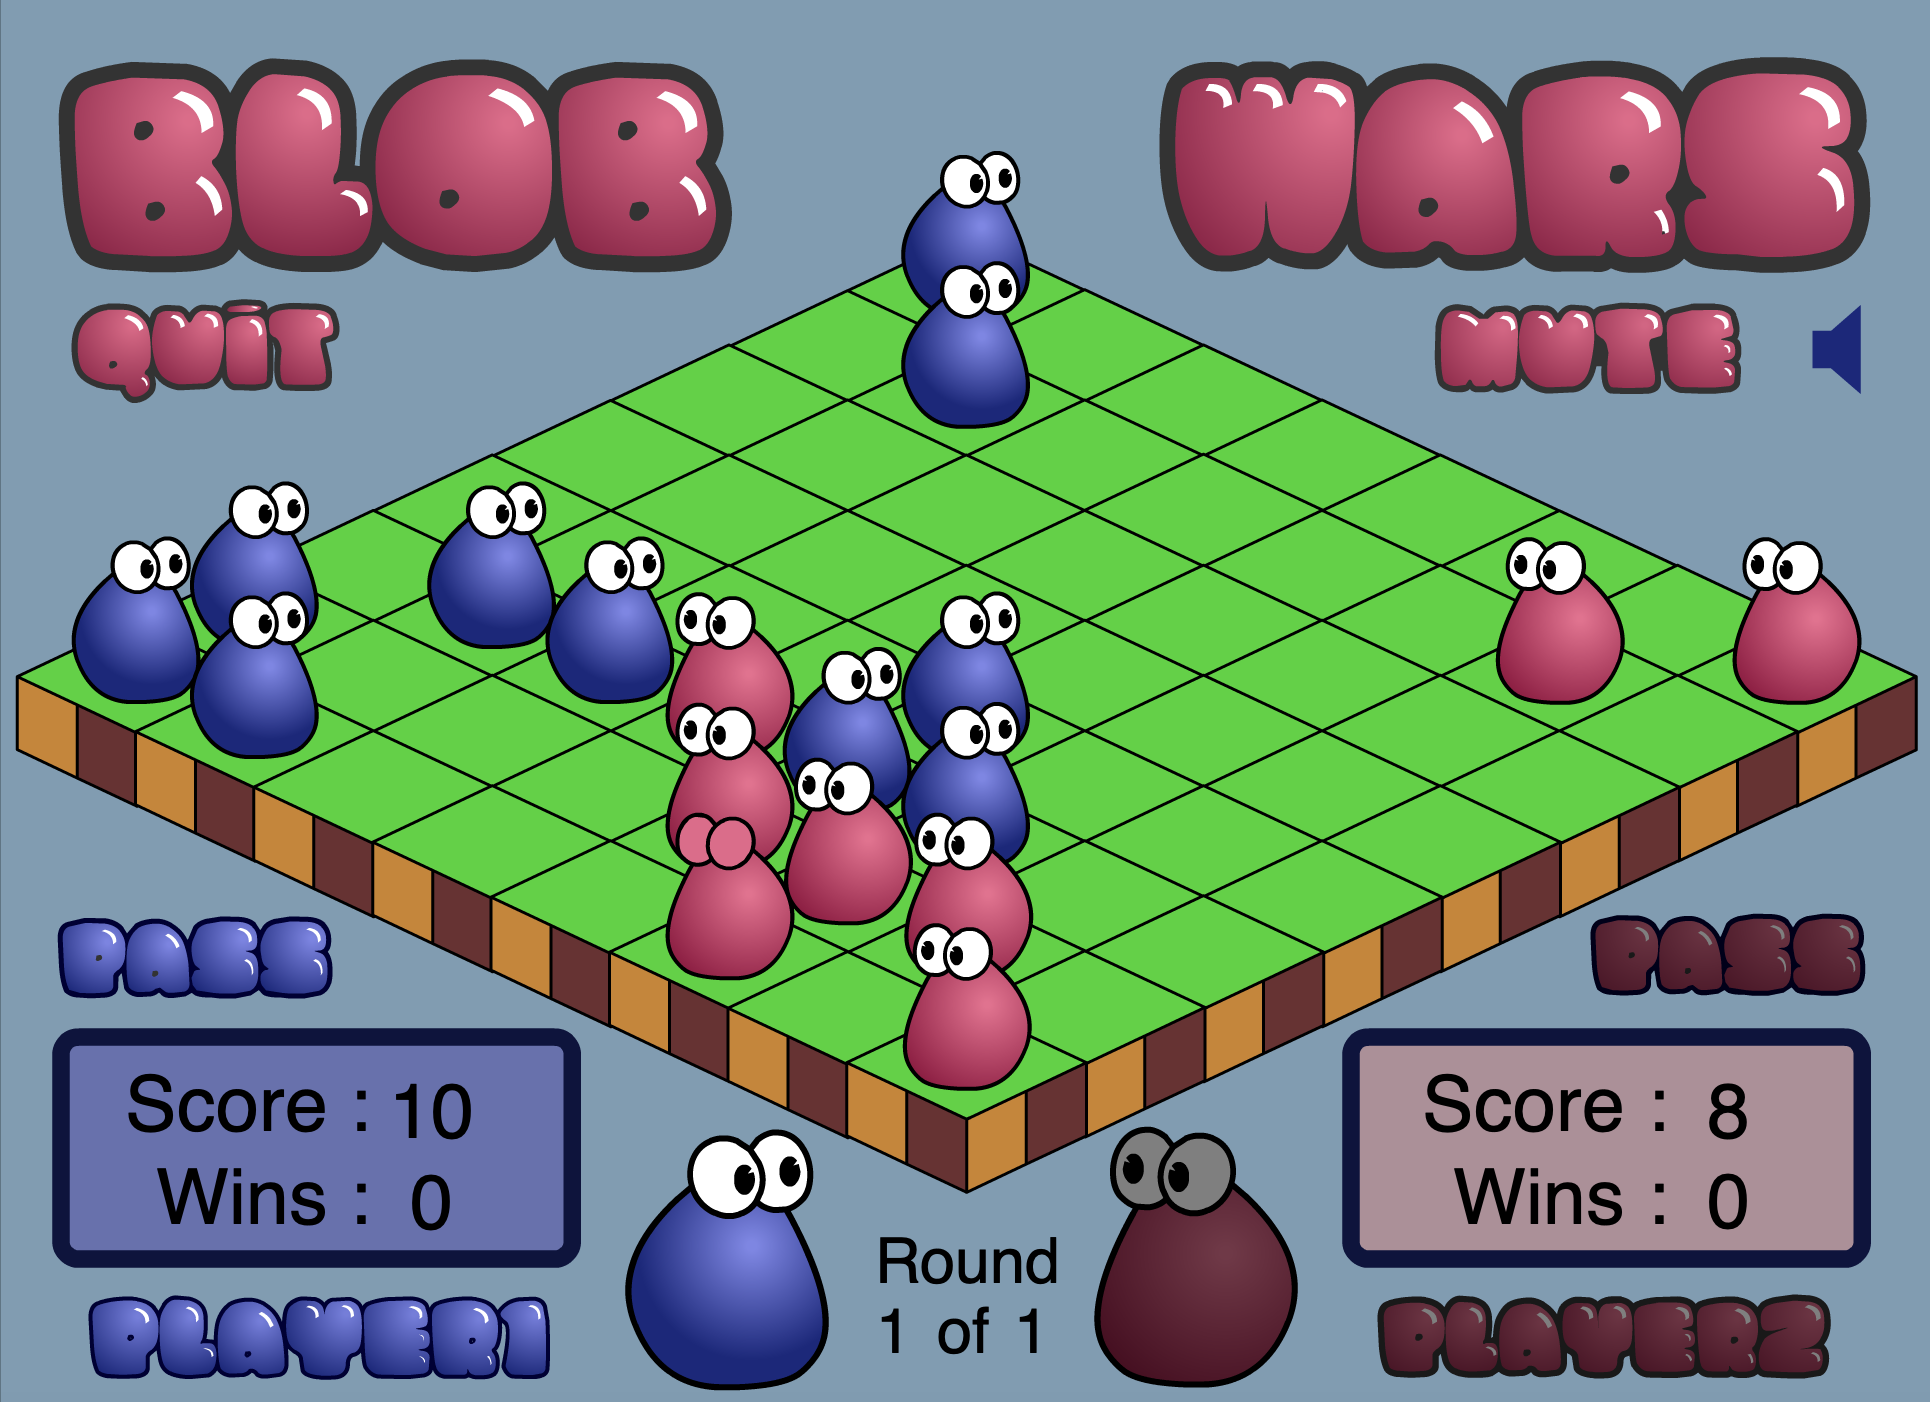
\includegraphics[width=0.95\textwidth]{figures/capture_ecran}
\caption{Capture d'écran d'un Blob Wars classique}
\label{fig:Screenshot1}
\end{center}
\end{figure}


\setcounter{section}{0}
\vspace{-10px}
\section{Choix des outils de développement}

Pour permettre un bon travail d'équipe, nous utilisons un espace de travail collaboratif GitLab\footnote{Site internet de GitLab : https://about.gitlab.com/.}\footnote{Page Wikipédia de GitLab : https://fr.wikipedia.org/wiki/GitLab\_CE.}\footnote{Lien vers le GitLab du projet : https://gitlab.info-ufr.univ-montp2.fr/e20170000656/Blob\_Wars\_HLIN405}  (\textsc{Figure}~\ref{fig:Logo1} en page 4) afin de nous organiser plus facilement en nous répartissant le travail. Cela permet de sécuriser l'avancée de notre travail en faisant des sauvegardes régulières depuis différents ordinateurs et dans différents lieux.\\

Nous gardons également une trace des tâches qu'il nous reste à accomplir et que nous avons déjà accomplies grâce à un diagramme de Gantt. Notre espace GitLab est hébergé par l'Université de Montpellier et est accessible par l'ensemble des membres du projet qui peuvent y faire des modifications.\\

\newpage

\begin{figure}[h]
 \begin{minipage}{.45\linewidth}
  \centering\epsfig{figure=figures/gitlab,width=\linewidth}
\caption{Logo du système de gestion GitLab \label{fig:Logo1}}
 \end{minipage} \hfill
 \begin{minipage}{.47\linewidth}
 \vspace{21px}
  \centering\epsfig{figure=figures/eclipse.png,width=\linewidth}
  \caption{Logo de l'IDE Eclipse \label{fig:eclipse}}
 \end{minipage}
\end{figure}

\vspace{20px}

Nous codons le Blob Wars en Java 8 conjointement avec la librairie Slick\footnote{Slick2D est une version arrangée pour développer des jeux en 2D facilement} sur l'IDE\footnote{Environnement de Développement Intégré} (\textsc{Figure} \ref{fig:eclipse}). Notre projet est suivi par M. Stéphane Bessy\footnote{Toutes les informations le concernant se trouvent sur https://www.lirmm.fr/~bessy/} que nous remercions pour son soutien, ses conseils et sa présence lors de nos réunions bimensuelles dont vous pouvez trouver les comptes-rendus en Annexe (pages 25 à 34).\\

M. Bessy est maître de conférences en informatique à l’Université de Montpellier et enseignant au département info de la Faculté des Sciences. Il est membre de l'équipe \textbf{AL}gorithmes de \textbf{G}raphes et \textbf{Co}mbinatoire (AlGCo) du LIRMM.

\vspace{13px}

\section{Diagramme de Gantt}

Nous avons conçu un diagramme de Gantt (\textsc{Figure} \ref{fig:Screenshot4}) afin de nous organiser dans le développement, mieux gérer le temps disponible et les échéances.

\vspace{10px}

\begin{figure}[htbp]
\begin{center}
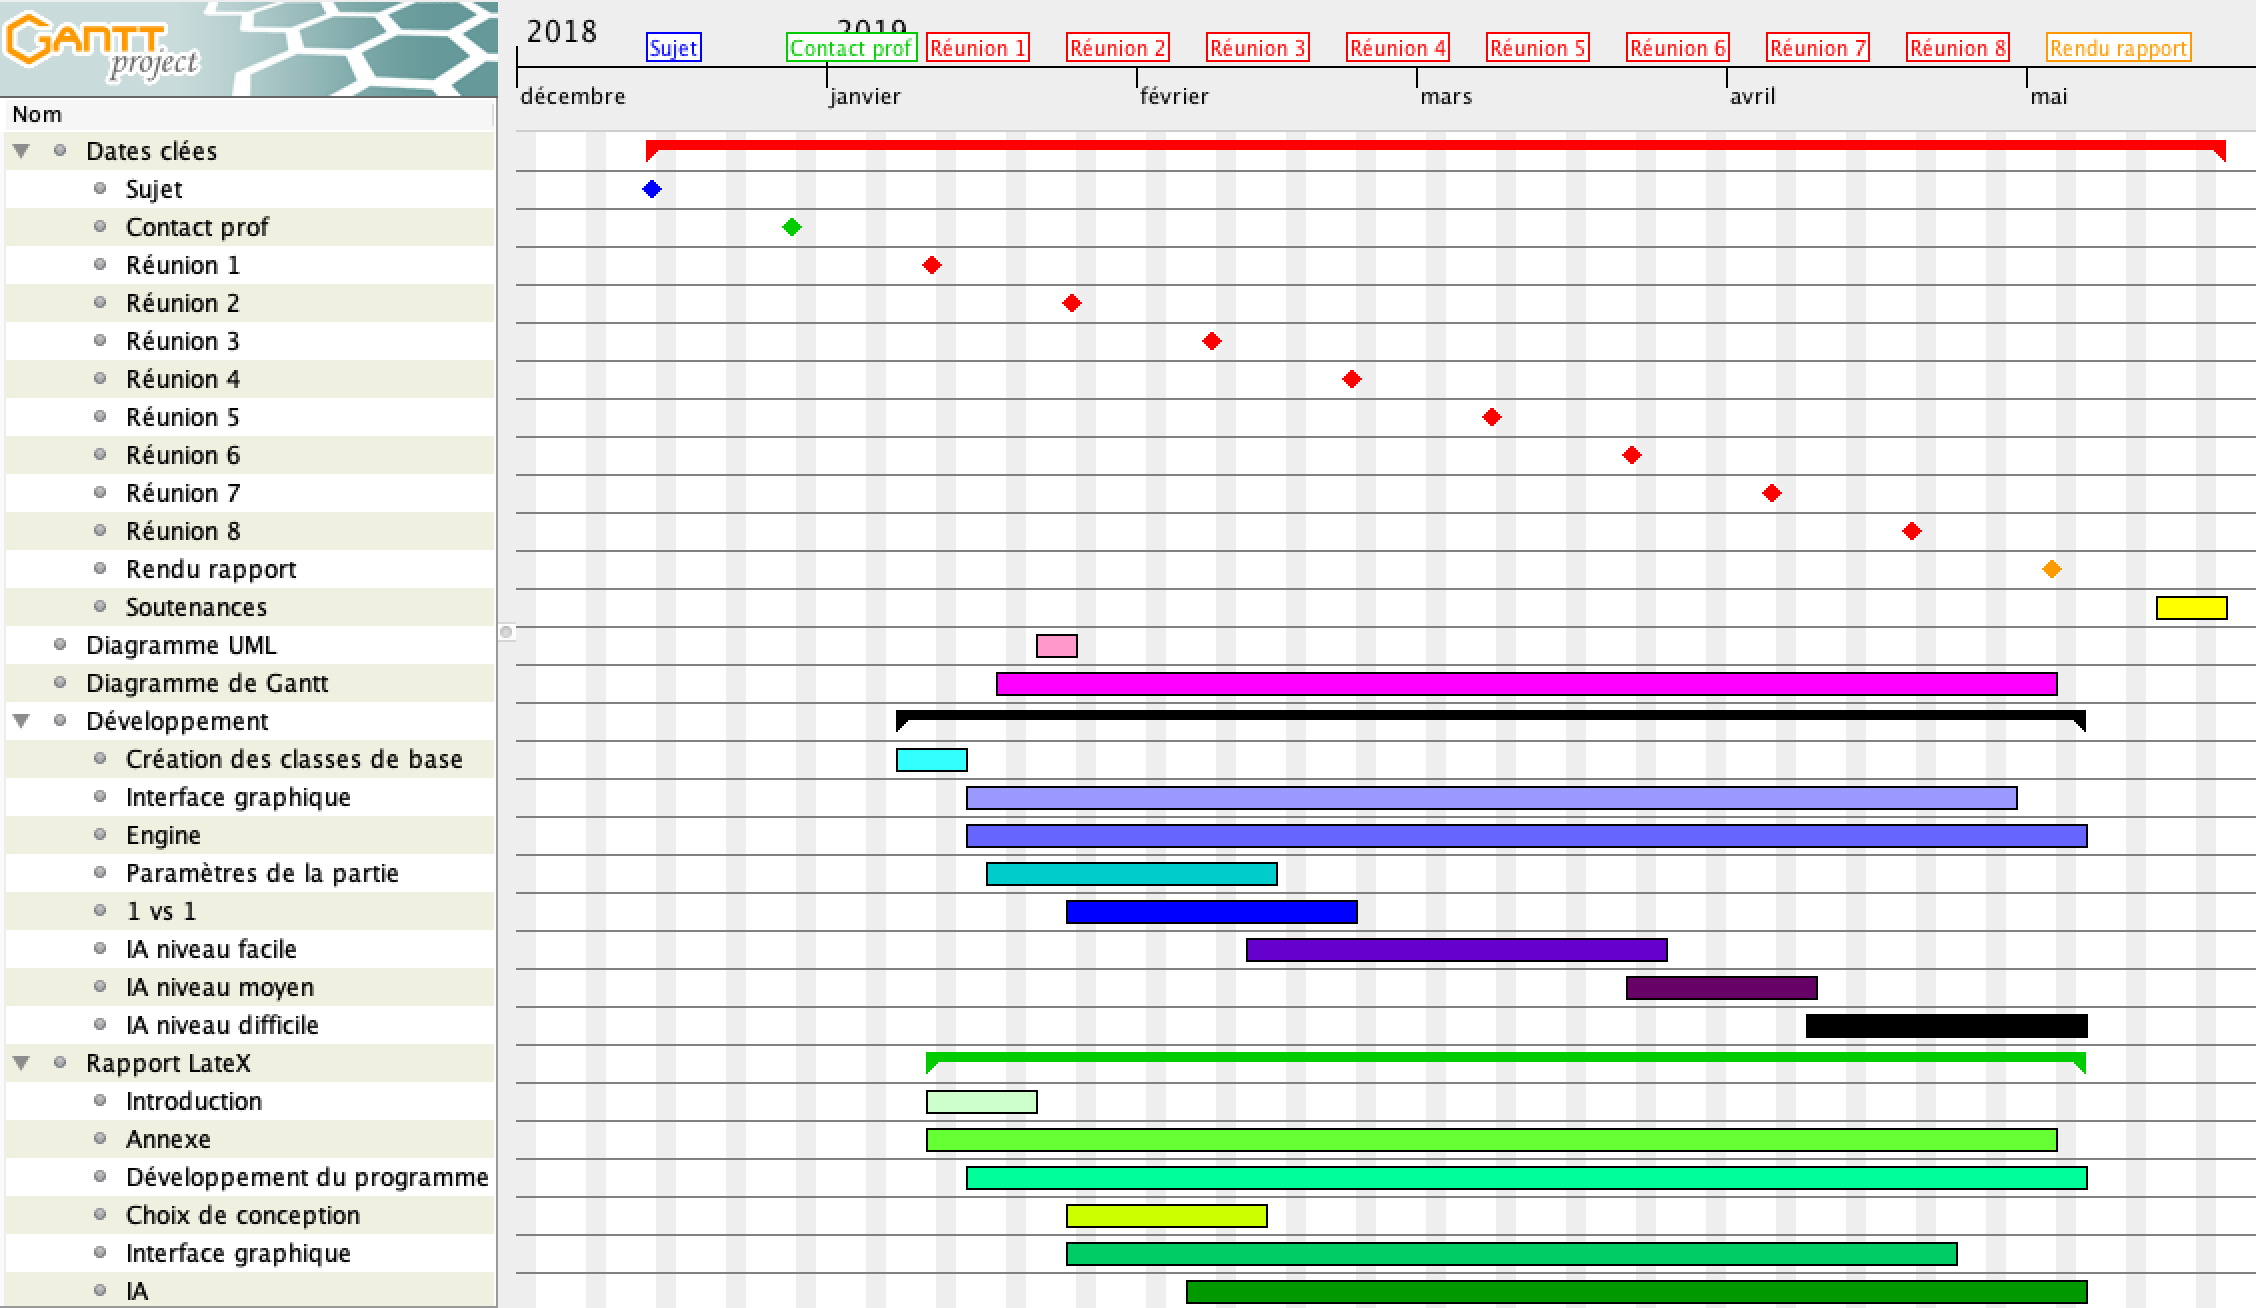
\includegraphics[width=1\textwidth]{figures/gantt}
\caption{Diagramme de Gantt initial}
\label{fig:Screenshot4}
\end{center}
\end{figure}

\newpage

\section{Règles du jeu}
\vspace{14px}
\begin{description}[itemsep=20pt]
    \item[Objectif:] Conquérir le plateau de jeu en attaquant les pions ennemis en les convertissant en vos pions.
    \item[Comment jouer:] Vous pouvez à chaque tour faire apparaître un pion ou déplacer un de vos pions déjà présent. 
    \begin{itemize}
        \item  Sélectionner un pion de votre équipe avec votre souris, le pion choisi sera mis en surbrillance et les déplacements possibles aussi (en nuances de gris) :
        \begin{itemize}[label=\textbullet]
            \item Sélectionner une case gris foncé (adjacente à votre pion) pour le dupliquer sur cette case.
            \item Sélectionner une case gris clair (adjacente à une case adjacente à un de vos pion) pour le déplacer sur cette case.
        \end{itemize}
        \item Chaque pion ennemi adjacent à la case sur laquelle vous vous êtes déplacé ou dupliqué sera converti en votre pion.
        \label{item:regle}
    \end{itemize}
    
    \item[Comment gagner:] Le gagnant est celui qui a le plus de pion à la fin de la partie. Convertir tous les pions du plateau est également une condition de victoire.
    
    \item[Fin de la partie:] Elle intervient une fois que le plateau est complètement rempli ou quand $n - 1$ joueurs ne peuvent plus jouer (où $n$ est le nombre de joueurs au total).
    
    \item[Egalité:] Il y a égalité lorsqu'à la fin de la partie plusieurs joueurs ont le (même) meilleur score. 
    \item[Passage automatique du tour:] Lorsque vous ne pouvez effectuer aucun mouvement.
    \item[Plus de pions sur le plateau:] Vous ne pourrez plus jouer, la partie s'arrête là pour vous.
    \item[Equipes:] Le jeu se joue aussi par équipes de 1 à 3 joueurs (2 équipes minimum et 4 équipes maximum puisque 2 joueurs minimum et 4 joueurs maximum dans une partie):
    \begin{itemize}
        \item Un joueur qui n'est pas dans votre équipe est considéré comme un ennemi.
        \item Un joueur de votre équipe est considéré comme un allié dont les pions ne peuvent ni être contrôlés ni être convertis.
    \end{itemize}
\end{description}

\newpage
\part{Développement}
\setcounter{section}{0}


\section{Présentation du projet}

Le Blob Wars est un jeu-vidéo de type réflexion qui implique une grande part de programmation "applicative" qui est à ce jour la plus utilisée pour développer (sans mentionner l'utilisation des frameworks). Les langages les plus connus qui prennent en compte ce paradigme de programmation sont le Python, le C, le C++, le C\#, le JAVA, le VB, le JS, etc. Tout comme il existe plusieurs langages, il existe aussi différentes façons de concevoir une "application". Grâce à notre cursus universitaire nous avons abordé différents pans de la programmation :
\begin{itemize}
    \item impérative
    \item orientée objet
    \item parallèle
    \item fonctionnelle
    \item événementielle
    \item web
\end{itemize}

\vspace{10px}

Les différents langages associés à ces différents paradigmes\footnote{Certains paradigmes sont imbriqués les uns aux autres, on distingue des "niveaux"} sont favorisés dans le choix du développement d'une application.\\

Le Blob Wars est un jeu de réflexion. Un jeu est un enchaînement d'événements qui peuvent influer certains objets du jeu qui vont à leur tour relancer un événement et ainsi de suite jusqu'à ce qu'un état final soit atteint. Chaque événement peut être modélisé comme une suite d'étapes qui sont associées à un comportement, à une entrée et qui \textit{ne change pas}\footnote{Sauf si c'est son objectif...}. Pour le dire autrement, on décrit un algorithme qui permet de traiter un état donné. Si on résume les différents points de notre projet, on y retrouve :

\begin{itemize}
    \item Des objets
    \item Des événements
    \item De l'impératif/procédural
\end{itemize}

\vspace{10px}

Voici un tableau (\textsc{Table} \ref{tab:tableauChoixLangages}) qui regroupe les pour et contre en fonction des langages qui nous sont connus\footnote{Que ce soit de nom ou par une utilisation pratique} et de nos critères. \\

\begin{table}[htbp]
    \centering
    \begin{tabular}{|*{4}{c|}}
      \hline
      Langages & Objets & Events & Utiliser\\
      \hline
      C & - & NA & +\\
      \hline
      C++ & + & + & +\\
      \hline
      C\# & + & + & -\\
      \hline
      Java & + & + & +\\
      \hline
      JavaScript & + & + & + \\
      \hline
      PHP & + & + & +  \\
      \hline
      Python & + & + & + \\
      \hline
      Ruby & + & + & - \\
      \hline
      Perl & + & + & -\\
      \hline
    \end{tabular}\\
    \label{tab:tableauChoixLangages}
    \caption{Comparatif des langages possibles}
\end{table}

\newpage

Au moment du choix du langage, une application web n'était pas considérée à cause de la taille du jeu. Ce qui ressort c'est donc C++, Java et Python. Cependant, nous avons décidé de commencer à programmer en Java car nous l'étudiions au même moment. De plus, Java permet de construire du code structuré et facilement modifiable.

\section{Objectif}

Le but principal de ce sujet de TER est l'intégration d'une Intelligence Artificielle (IA). On va implémenter cette IA grâce à des algorithmes comme notamment :
\begin{enumerate}
    \item le MinMax (parcourt d'un arbre et choix de la branche la plus optimale)
    \item l'Alpha-Bêta (élagage de l'arbre parcouru par le MinMax et diminution du temps de calcul)
\end{enumerate}

\section{Structure des principales classes du programme}

\subsection{Dossier $Slick$}

Il s'agit ici de la gestion de l'interface graphique. Toutes ces classes sont des éléments affichés.

\begin{itemize}
    \item \textbf{Menu :}
    \begin{itemize} [label=$\Rightarrow$]
    \item Contient des boutons qui permettent l'accès au lancement du jeu, l'aide, les crédits, les options ou encore quitter.
    \end{itemize}
    
    \item \textbf{Options :}
    \begin{itemize} [label=$\Rightarrow$]
    \item Contiendra la possibilité de changer le volume de la musique et des bruitages.
    \item Boutons pour quitter le jeu et y revenir.
    \end{itemize}

    \item \textbf{Game :}
     \begin{itemize} [label=$\Rightarrow$]
    \item Affiche les scores à gauche, individuels et par équipe ainsi que le plateau du jeu.
    \end{itemize}
    
    \item \textbf{Crédits :} 
    \begin{itemize} [label=$\Rightarrow$]
    \item Affiche un rectangle contenant toutes les informations concernant la création du projet.
    \end{itemize}
    
    \item \textbf{Aide :} 
    \begin{itemize} [label=$\Rightarrow$]
    \item Fenêtre très similaire à celle de Crédits, mais qui affiche des informations concernant l'utilisation de ce programme.
    \end{itemize}
    
    \item \textbf{Bouton :}
    \begin{itemize} [label=$\Rightarrow$]
    \item Facilite l'ajout de boutons dans une fenêtre.
    \end{itemize}
    
    \item \textbf{Slide :}
    \begin{itemize} [label=$\Rightarrow$]
    \item Facilite l'ajout de "slide" dans une fenêtre (la barre de volume par exemple).
    \end{itemize}
    
\end{itemize}

\subsection{Dossier $Engine$}

Il s'agit d'une classe qui permet les autres calculs graphiques liés au programme.

\begin{description}[itemsep=5pt]
    \item[Case:] Une case contient sa position, sait si un joueur l'occupe et si elle est accessible.
    \item[Damier:] Classe contenant un tableau de deux dimensions de cases, c'est donc le jeu
    \item[Joueur:] Une classe qui contient les informations du joueur, son nom, son score, son équipe,...
    \item[IA:] Une classe qui renvoie le prochain coup à jouer pour un joueur et un état de jeu donné.
\end{description}

\newpage

\section{Structure globale}
    
\begin{figure}[h]
\begin{center}
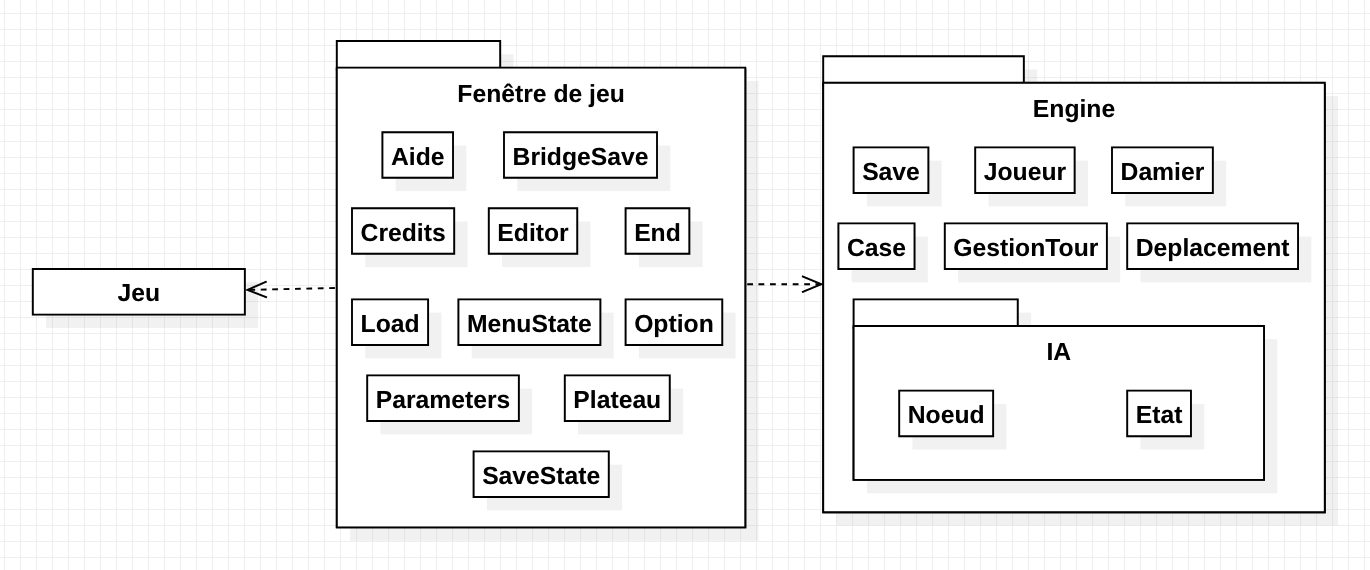
\includegraphics[width=1\textwidth]{figures/diagramme_simp.png}
\caption{Diagramme de classes simplifié global}
\label{fig:global}
\end{center}
\end{figure}

La structure de notre jeu Blob Wars est composée d'une fenêtre de jeu (interface graphique) qui dialogue avec le moteur du jeu ainsi que le jeu en lui-même (voir \textsc{Figure} \ref{fig:global}). Vous pouvez retrouver des diagrammes de classes plus globaux et détaillés en Annexe (pages 20 à 22).

\section{Icône, "blobs", musique et bruitages}

Nous avons créé une icône pour l'application (voir \textsc{Figure} 6). Dans notre version du Blob Wars, les "blobs" sont des logos de moteurs de recherche ou de systèmes d'exploitations. La musique du jeu Blob Wars ainsi que tous les bruitages ont été composés et réalisés à l'aide du logiciel de MAO\footnote{Musique Assistée par Ordinateur} Garage Band\footnote{Site internet de Garage Band : https://www.apple.com/fr/mac/garageband/}.

\vspace{10px}

\begin{figure}[h]
\begin{center}

\includegraphics[width=0.4\textwidth]{figures/icone.png}
\caption{Icône de l'application Blob Wars}
\end{center}
\end{figure}

\newpage

\section{Fichier de configuration}

L'utilisateur a la possibilité de générer et charger des fichiers de configuration afin de sauvegarder ou charger des parties. Chaque fichier de configuration représente l'état d'une partie. Les fichiers sont générés de la manière suivante (voir \textsc{Figures} 7 et 8) : 
\begin{description}[itemsep=3pt]
    \item[La date et l'heure :] Sur une ligne (ici l.1).
    \item[Le nombre de joueurs : ] Sur une ligne (ici l.3).
    \item[Les propriétés des joueurs :] Sur autant de lignes qu'il y a de joueurs. L’index, la mention joueur, le nom, l’équipe, l’avatar et son index d’avatar, y sont précisés pour chaque joueur physique. Dans le cas d’une IA, la mention joueur est remplacée par le niveau de l’IA. Il y a donc autant de lignes que de joueurs au total (ici l.5 à 8).
    \item[L'index du joueur qui doit jouer :] Sur une ligne (ici l.9).
    \item[La taille du plateau de jeu :] Sur une ligne (ici l.11).
    \item[Le plateau :] Sur une ligne. Chaque numéro correspond à l'index du joueur. Le chiffre zéro représente une case vide et la lettre X une case inaccessible (avec des murs) (ici l.13 à 20).
\end{description}

\begin{figure}[htbp]
\begin{lstlisting}[style=mystyle]
2019/04/02 00:23:58

4

1 tres_facile Joe red firefox 2
2 joueur William blue ie 5
3 moyen Jack green windows 6
4 joueur Averell yellow chrome 4
2

8

11000400
11004400
100XX000
30XXXX02
00XXXX20
000XX020
30000000
30000000
\end{lstlisting}

\caption{Exemple d'un fichier de configuration}
\label{fig:config1}
\end{figure}

\begin{figure}[h]
\begin{center}
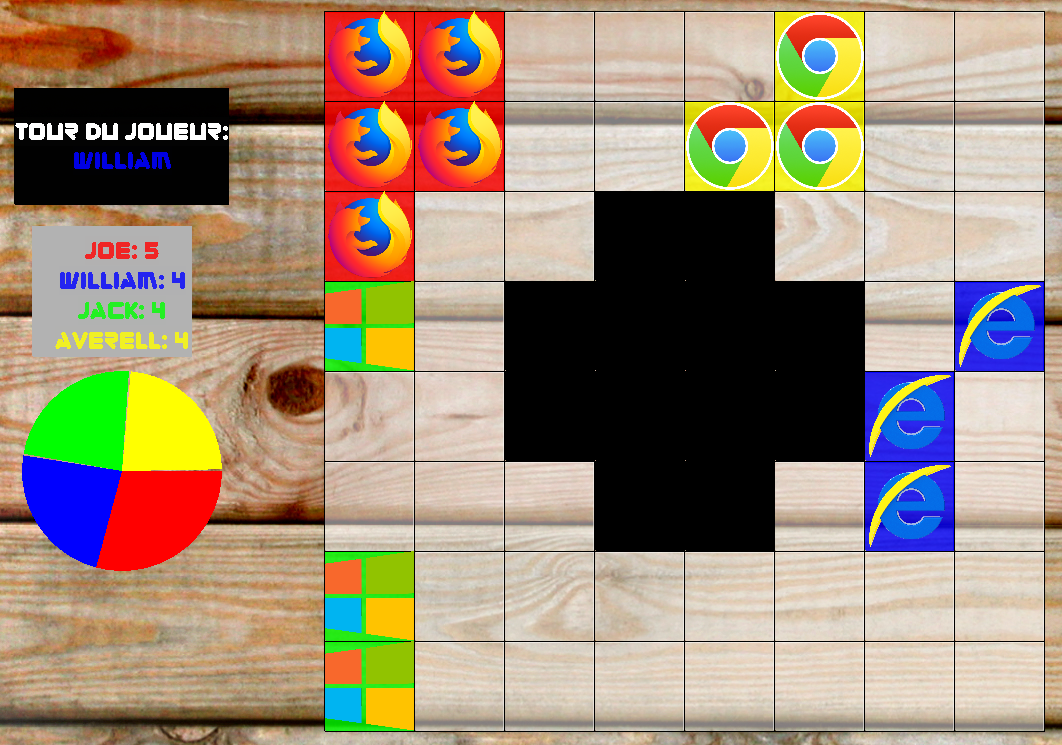
\includegraphics[width=0.46\textwidth]{figures/capturejeu.png}
\caption{Capture d'écran de la partie correspondant au fichier de configuration de la \textsc{Figure} 7}
\label{fig:config2}
\end{center}
\end{figure}

\newpage

\part{Intelligence artificielle}

\setcounter{section}{0}

\section{IA minmax}

\subsection{Fonctionnement de la classe}

La classe IA est un peu spéciale car elle ne devient une instance qu'une seule fois\footnote{C'est ce que l'on appelle un singleton. Cela garanti qu'une unique instance d'une classe donnée sera créée et offre un point d'accès universel à cette instance.} . À profondeur égale, une IA agit toujours de la même façon face à une situation de jeu donnée. Elle contient les méthodes nécessaires au calcul du prochain coup.

\subsection{Méthodes de la classe IA}

\begin{description}[itemsep=5pt]

    \item[eval:] Permet à partir d'un état de jeu et d'un joueur, de lui attribuer une valeur qui qualifie sa chance de victoire. Cette fonction n'est appelée que sur les feuilles.
    
   \item[simulerCoupDePosition:] Permet à partir d'une case de jeu, de fournir tous les coups que le pion situé au-dessus peut effectuer, donc les cases accessibles autour de cette même case.
    
    \item[simulerTousLesCoups:] Chaque état de jeu contient les positions des joueurs, il suffit pour chacune de leur position de calculer tous leurs coups possibles.

    \item[min et max:] Deux fonctions qui à partir d'une liste d'état, nous renvoie soit le meilleur état pour le joueur dans le cas de max, soit le pire dans le cas de min.
    
    \item[minimax:] Renvoie le meilleur coup que le joueur peut effectuer (en créant l'arbre des possibilités par récursion et le remontant en appliquant le max ou min si c'est le tour d'un ennemi ou d'un allié).
\end{description}

On remarque que l'algorithme MinMax n'est pas assez optimal en temps de calcul et nous utiliserons donc l'élagage Alpha-Bêta du MinMax pour gagner du temps de calcul.\\

\subsection{Implémentation de l'algorithme MinMax}

\vspace{5px}

Voici le pseudo-code produit à partir de notre implémentation du minimax (\textbf{Algorithme 1} en page 11).\\

Le cas de base correspond à une feuille de l'arbre des différentes parties ici identifiée par \textbf{profondeur >= 0 et JeuPasFini}. Dans les autres cas, si c'est notre tour, on va calculer le coup qui nous fait gagner le plus de points\footnote{En fonction d'une fonction d'évaluation (ici appelée \textbf{calculerValeurEtatJeu})}. Sinon on cherche à calculer le meilleur coup pour l'adversaire c'est à dire le minimum de notre point de vue.\\

Cette opération est répétée pour toutes les cases autour de notre pion et on simule autant de coups pour chacune de ces cases là que de profondeur choisies pour notre algorithme. Cela donne une complexité en $\theta(n^p$) avec $n$ le nombre de coups possibles pour une position et $p$ la profondeur de calcul.\\

Pour expliquer cela, un schéma est le moyen le plus adapté. Au lieu d'en refaire un, nous utilisons celui disponible sur la page Wikipédia de l'alpha-bêta et que vous pourrez retrouver sur la \textsc{Figure} 9 en page~\pageref{fig:alphabeta} dont il faut ignorer les élagages. Vous trouverez en Annexe (page 23) plusieurs courbes de temps d'exécution du MinMax pour lesquelles on fait varier le nombre de joueurs, la profondeur des IA et la taille de la zone de jeu.

\newpage

\vspace{20px}

\begin{algorithm}[H]
\Variables{$monTour?$ : booléen, $tourEquipe?$ : booléen, $joueurActuel$ : entier}
$monTour? \gets (joueurActuel = joueur)$\;
$tourEquipe? \gets $ estAllieA($joueur$)\;
simulerTouslesCoups()\;
$profondeur \gets profondeur-1$\;
tourSuivant()\;
\eSi{$profondeur >= 0$ \KwEt JeuPasFini} {
    \Pour{i \KwDe $0$ \KwA nbNoeud}{
        \Si{minMax($joueur$, $gestionTour$, $noeudCourant$, $noeudCourant$) $= null$} {
        Fin du calcul\;
        }
    }
    \eSi{monTour? \KwOu tourEquipe?} {
    Le $noeudChoisi$ prend la valeur du maximum de tous les nœuds\;
    $noeudCourant \gets noeudChoisi$\;
        \Si{$noeudPere \neq null$} {
        $noeudPere.alpha \gets max(noeudChoisi,noeudCourant.alpha)$\;
        }
        \Si(\tcp*[f]{Elagage alpha/beta}){$noeudCourant.beta \le noeudCourant.alpha$} { 
        \Kwrenv $null$\;
        }
    }
    {
     Le $noeudChoisi$ prend la valeur du minimum de tous les nœuds\;
    $noeudCourant \gets noeudChoisi$\;
    \Si{$noeudPere \neq null$} {
        $noeudPere.beta \gets min(noeudChoisi,noeudCourant.beta)$\;
        }
    \Si(\tcp*[f]{Elagage alpha/beta}){$noeudCourant.beta \le noeudCourant.alpha$} {
    \Kwrenv $null$\;
    }}
}
{$noeudCourant \gets $ calculerValeurEtatJeu($joueur$)\;}
\Kwrenv $noeudChoisi$\;
\caption{minMax ($joueur$ : entier, $gestionTour$ : GestionTour, $noeudCourant$ : Noeud, $noeudPere$ : Noeud) : Etat}

\label{algo:max}
\end{algorithm}

\vspace{20px}

\section{Heuristique}

Dans cette section nous analysons empiriquement et sans outils de précision les données mesurées lors de nos phases de test (pendant le développement).
\begin{itemize}
    \item Temps moyen du tour pour un joueur humain : quelques dizaines de secondes.
    \item Temps moyen de l'algorithme sur un plateau 6x6 jusqu'à 10x10 : de quelques secondes à quelques minutes sans élagage du MinMax, de quelques secondes à quelques dizaines de secondes avec élagage (voir partie suivante à propos de l'élagage)
\end{itemize}

\vspace{10px}

Des tests plus détaillés et plus précis que ceux de la \textsc{Table} 2 (page 12) sont disponibles en Annexe (page \pageref{fig:minMaxTempsExecution}). Ils montrent le besoin d'optimiser cet algorithme afin de diminuer le temps de calcul.

\newpage

\begin{table}[htbp]
    \centering
    \begin{tabular}{|l|c|c|c|c|c|}
        \hline
         Algorithme & profondeur & quelques sec. & dizaines de sec. & quelques min. & infinie \\
         \hline
         MinMax & 1 & x & x & &\\
         \hline
         MinMax & 2 & x & x & &\\
         \hline
         MinMax & 3 &  & x & x &\\
         \hline
         MinMax & 4 &  & x & x &\\
         \hline
         MinMax & 5 &  &  & x & x\\
         \hline
         MinMax & 6 &  &  &  & x\\
         \hline
    \end{tabular}
    \label{tab:tableauComparaisonTempsCalculCoup}
    \caption{Observation du temps de calcul de chaque coup pour chaque algorithme implémenté}
\end{table}

\section{Élagage alpha-bêta}

Comment optimiser l'algorithme MinMax ? C'est la question que certains informaticiens se sont posées et dont ils ont trouvé la solution.

\subsection{Compréhension de cet élagage}

L'objectif de cette optimisation est de couper (ou élaguer) les branches de notre arbre pour avoir moins de contenu à explorer. Qui dit moins de contenu à explorer dit moins de calculs à effectuer.
Cette opération est communément appelée un élagage. Cet élagage est très utilisé car il permet de n'avoir aucune perte d'informations (et ainsi perdre aucun meilleur coup) tout en diminuant le nombre de calculs à effectuer. Il est implémenté par les lignes dont les 
commentaires sont explicites dans l'\textbf{Algorithme 1} (page 11).

\subsection{Illustration de son fonctionnement sur un exemple}

\begin{figure}[h]
\begin{center}
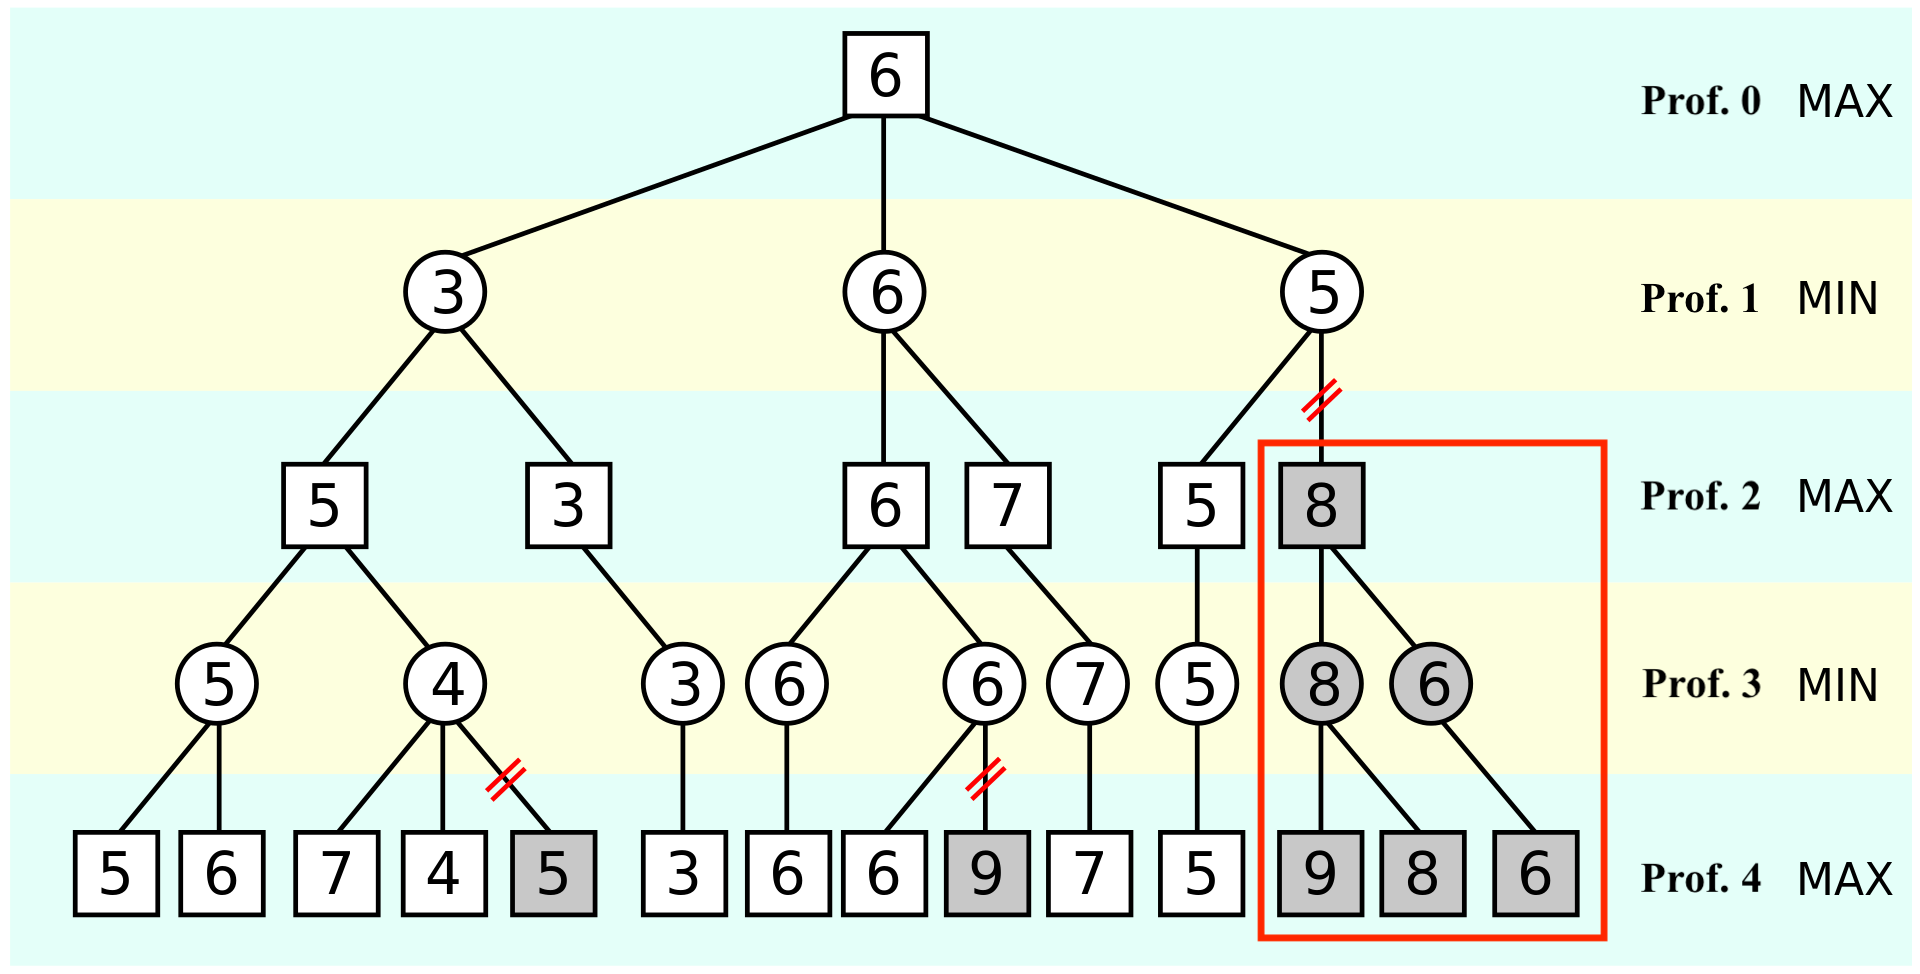
\includegraphics[width=0.9\textwidth]{figures/elagage/alphabeta.png}
\caption{Exemple d'un arbre étiqueté avec les valeurs d'un MinMax avec élagage alpha-bêta}
\label{fig:alphabeta}
\end{center}
\end{figure}

Sur la \textsc{Figure} \ref{fig:alphabeta}, on constate que plusieurs coupures ont été réalisées. On étudie l'élagage du sous-arbre encadré en rouge. Le nœud MIN (profondeur 1) vient de mettre à jour sa valeur courante à 5. Celle-ci, qui ne peut que baisser, est déjà inférieure à $\alpha=6$, la valeur actuelle du nœud MAX précédent (profondeur 0). Ce nœud MAX cherchant la valeur la plus grande possible, il ne la choisira donc pas de toute façon. On peut donc stopper le parcours du MinMax en élaguant avec l'implémentation alpha-bêta du MinMax le sous-arbre encadré en rouge.

\newpage

\subsection{Calculs de temps d'exécution à partir de l'implémentation de l'alpha-bêta}

\begin{figure}[h]
\begin{center}
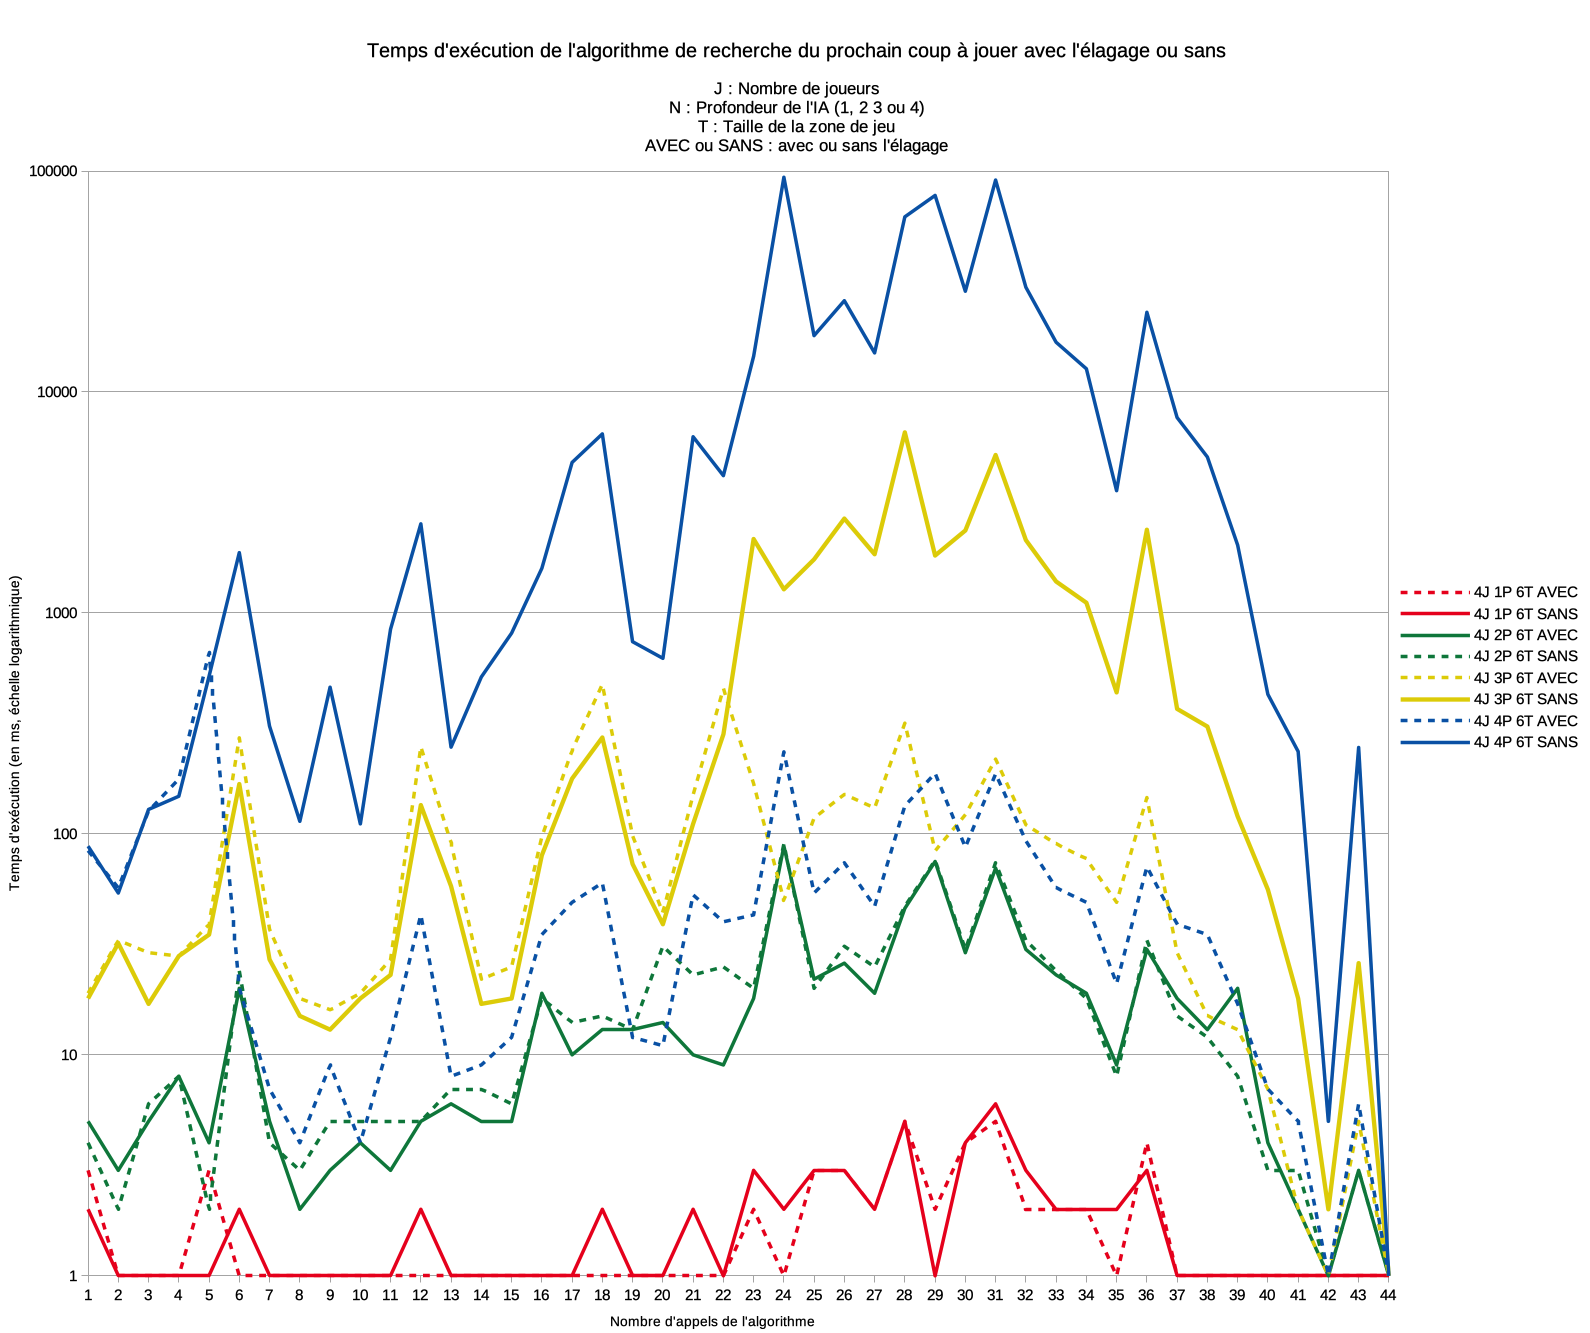
\includegraphics[width=1\textwidth]{figures/elagage/alphabetacourbe.png}
\caption{Exécution de l'algorithme MinMax avec élagage alpha-bêta ou non}
\label{fig:creer}
\end{center}
\end{figure}

On exécute le programme pour 4 joueurs et une taille de terrain de 6 cases de côté. On fait varier la profondeur de l'IA de 1 à 4 et on active (courbe en pointillé) ou pas (courbe avec trait continu) l'élagage. On rassemble les résultats sur la \textsc{Figure} 10. On constate que :

\vspace{10px}

\begin{itemize}[5px]
    \item Pour les profondeurs 1 et 2 (courbes rouges et vertes), l'élagage ne fait quasiment pas varier le temps d'exécution de l'algorithme par rapport aux courbes sans l'élagage à ces profondeurs.
    \item Pour la profondeur 3 (courbes jaunes), l'élagage fait gagner un peu de temps d'exécution notamment au moment de l'explosion de calcul (autour de l'appel numéro 22 de la courbe jaune continue). Mise à part que cette explosion de calcul correspond au passage à 2 joueurs, nous n'avons pas d'explication plus précise quand à ce phénomène.
    \item Pour la profondeur 4 (courbes bleues), l'élagage est encore plus bénéfique en temps de calcul que précédemment. Le temps d'exécution à cette profondeur est voisin des courbes de profondeur 3.
    \item Suite à d'autres tests, nous constatons que le gain de temps de l'élagage est d'autant plus important que la profondeur de l'IA grandit.
\end{itemize}

\newpage

\part{Aperçu du jeu}

Voici maintenant une présentation des principales fenêtres de l'application ainsi que de leur utilité.\\

Sur la \textsc{Figure} 11, voici une capture d'écran du menu de création d'une partie. L'utilisateur peut définir le nom et le nombre de joueurs ou IA (et leur niveau) à l'aide de l'interface. Il y a également possibilité de changer la taille de la carte et de jouer sur des cartes ayant des murs ou pas. Il existe également un éditeur de carte (Figure 14) accessible depuis ce menu.\\

\begin{figure}[h]
\begin{center}
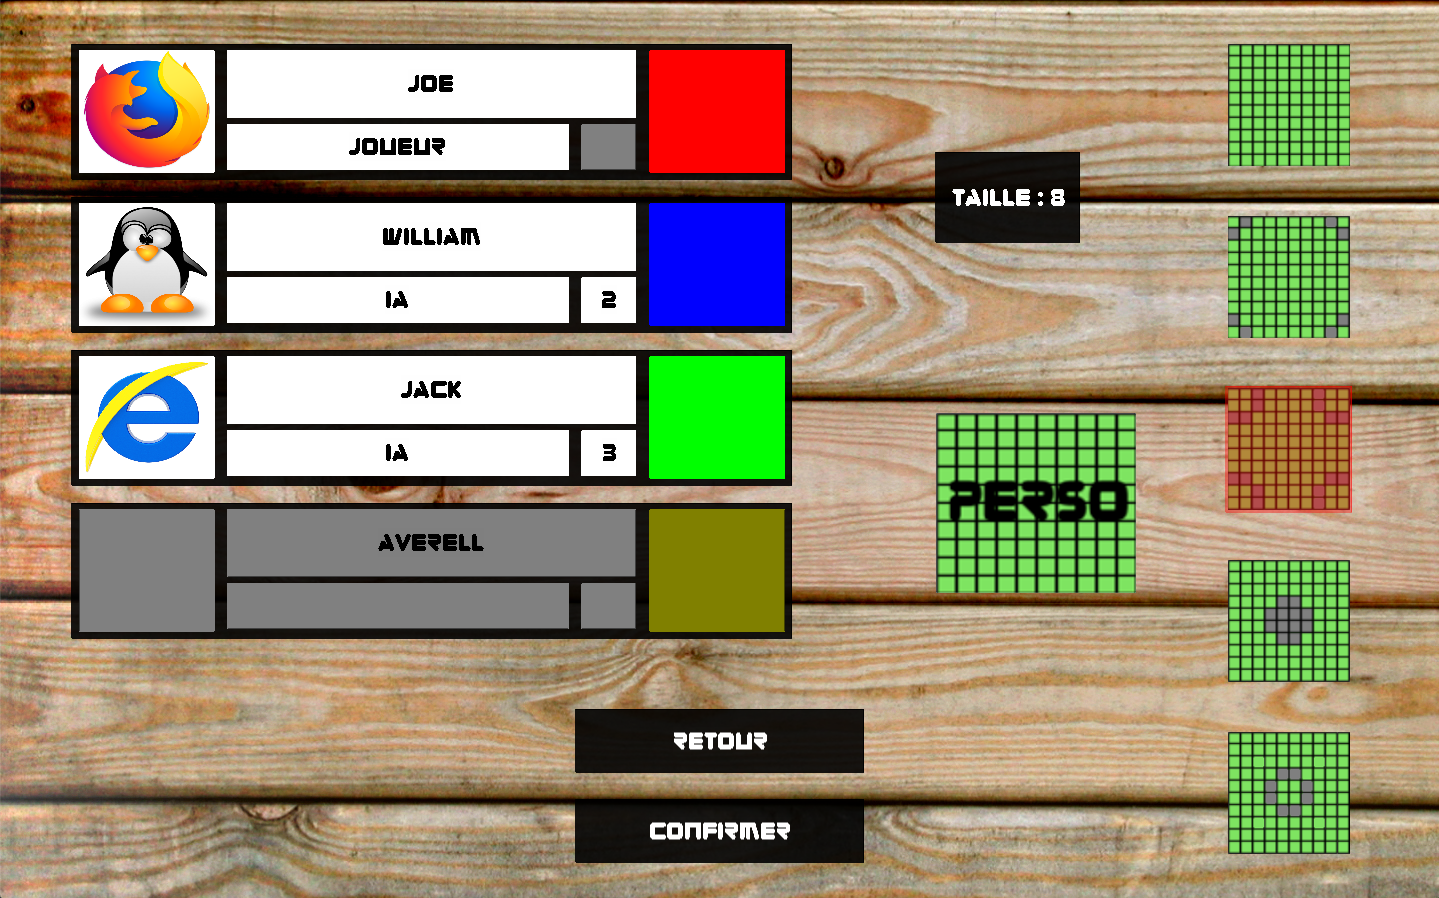
\includegraphics[width=1\textwidth]{figures/captureJeu/captureCreer.png}
\caption{Création d'une partie}
\label{fig:creer}
\end{center}
\end{figure}

Les \textsc{Figures} 12 à 17 sont situées sur la page suivante.\\

La \textsc{Figure} 12 est une capture d'écran du menu principal depuis lequel on a accès au bouton JOUER qui permet de créer ou charger une partie (\textsc{Figure} 14). Le bouton AIDE dirige vers une fenêtre qui explique comment utiliser l'application. Le bouton OPTIONS permet d'accéder au menu présenté en \textsc{Figure}. Le bouton CREDITS permet d'accéder aux crédits et le bouton QUITTER permet de quitter l'application.\\

Pendant une partie (\textsc{Figure} 16) on peut accéder au menu pause (\textsc{Figure} 13) avec la touche \textit{Echap} du clavier afin de changer indépendamment le volume de la musique ou des bruitages (réalisés par nos soins). Lorsque la partie est terminée (\textsc{Figure} 17), on peut accéder au menu principal du jeu.

\begin{figure}[H] 
 \begin{minipage}[b]{.46\linewidth}
  \centering\epsfig{figure=figures/captureJeu/captureMenu.png,width=\linewidth}
  \caption{Menu principal \label{fig:Menu}}
 \end{minipage} \hfill
 \begin{minipage}[b]{.46\linewidth}
  \centering\epsfig{figure=figures/captureJeu/captureOptions.png,width=\linewidth}
  \caption{Options sonores \label{fig:Options}}
 \end{minipage}
\end{figure}

\begin{figure}[H] 
 \begin{minipage}[b]{.46\linewidth}
  \centering\epsfig{figure=figures/captureJeu/captureLoad.png,width=\linewidth}
  \caption{Chargement et sauvegarde de parties \label{fig:Load}}
 \end{minipage} \hfill
 \begin{minipage}[b]{.46\linewidth}
  \centering\epsfig{figure=figures/captureJeu/captureMap.png,width=\linewidth}
  \caption{Éditeur de carte \label{fig:Map}}
 \end{minipage}
\end{figure}

\begin{figure}[H] 
 \begin{minipage}[b]{.46\linewidth}
  \centering\epsfig{figure=figures/captureJeu/capturePartie.png,width=\linewidth}
  \caption{Pendant une partie \label{fig:Partie}}
 \end{minipage} \hfill
 \begin{minipage}[b]{.46\linewidth}
  \centering\epsfig{figure=figures/captureJeu/captureFin.png,width=\linewidth}
  \caption{Fin d'une partie \label{fig:Fin}}
 \end{minipage}
\end{figure}

\newpage

\part{Conclusion}
\setcounter{section}{0}

    Mise à part programmer, un des objectifs du projet de programmation est de nous faire réfléchir à l'organisation de notre groupe, par exemple en utilisant un diagramme de Gantt et des outils de travail adaptés à nos besoins (comme Git, StarUML ou Eclipse).\\
    
    Cette phase de conception (de pré-traitement) définit un temps pendant lequel nous réfléchissons sans toucher à un ordinateur. C'est une étape importante dans notre projet, d'autant plus quand on se rend compte à posteriori le temps gagné à ce moment là. Pendant cette phase, nous avons décidé de choisir Jérémie comme porte-parole pour les interactions avec notre encadrant. Cette phase consistait à faire un état de l'art de l'informatique, c'est-à-dire des technologies ou langages qui sont utilisés pour faire un jeu-vidéo comme Blob Wars. Cette étape de réflexion était faite en groupe et nous discutions constamment des points à améliorer.\\
    
    À la suite de cela, nous avions un cahier des charges, un langage et un IDE. Nous avons ensuite créé un calendrier avec les différentes étapes du développement (un diagramme de Gantt, \textsc{Figure} 4 en page 4) que nous avons globalement respecté.\\
    
\section{Bilan}

    Pour résumer, nous avons développé un jeu-vidéo de type Othello appelé Blob Wars. Ce jeu-vidéo suit les règles précédemment énoncées en page \pageref{item:regle} et nous y avons ajouté la possibilité de jouer contre une IA qui suit l'algorithme du MinMax (voir page \pageref{algo:max}). Nous arrivions à des temps de calculs infinis pour nos machines (pour des profondeurs supérieures à 4) ce qui était d'autant plus mauvais quand on jouait contre une autre IA. C'est pourquoi, nous avons rapidement dû optimiser l'algo MinMax grâce à l'élagage alpha-bêta (voir page \pageref{fig:alphabeta}).\\
    
    En parallèle, nous avons utilisé le logiciel \textit{Sothink SWF Decompiler} pour récupérer l'algorithme du jeu donné dans le sujet. Nous avons alors découvert que l'IA du jeu Blob Wars en ligne était basée sur un enchaînement de boucles \textit {If/Else} (voir compte-rendu de la réunion du 18 mars en page \pageref{entrevue:18mars}).\\
    
\section{Compétences mises en œuvre}

    Grâce à ce TER, nous avons mis en pratique les connaissances acquises dans les modules d'\textit{Algorithmique et complexité} (HLIN401), \textit{Modélisation et programmation par objet 1} (HLIN406) et \textit{Programmation impérative avancée} (HLIN302). En effet, nous avons su analyser et construire des algorithmes complexes avec des structures de données complexes choisies en adéquation avec le langage JAVA et les thématiques rencontrées.\\
    
    Nous avons également sollicité des compétences du module \textit{Techniques de communication et conduite de projets} (HLIN408). Par exemple, nous rédigeons ce rapport en \LaTeX~avec l'application web \textit{Overleaf} et nous utilisons le logiciel \textit{Git} : nous savons maintenant maîtriser l'essentiel de ces 2 outils. Enfin, nous avons grandement favorisé l'utilisation de l'open-source et du gratuit dans la limite du possible.\\
    
    Ce TER a aussi été bénéfique sur le plan humain. Tout d'abord, au niveau de l'organisation du travail en groupe, le logiciel \textit{Discord} à l'aide duquel nous avons communiqué pendant le développement a permis de faciliter les choix et la répartition des tâches. Enfin, dialoguer (pas seulement à propos du TER) avec M. Bessy et les membres du groupe a permis de discuter orientation, projet professionnel et informatique en général. Chacun a appris des autres et de ses expériences.

\newpage

\section{Extensions et perspectives d'avenir}

    En date du 7 mai, voici une liste non-exhaustive de ce que nous souhaiterions implémenter en plus que ce qui avait été demandé (avec les difficultés et possibilités que cela ouvrirait si ces implémentations voyaient le jour):\\
    
    \begin{itemize}
        \item Un développement orienté web.
            \begin{enumerate}
                \item Une difficulté sur laquelle nous nous sommes mis d'accord réside dans le fait que le code que nous avons ne peut pas être simplement transposé dans un des langages web que nous avons précédemment vu, la conception du programme devant être revue.
                \item Cependant, cela serait fait avec l'objectif de pouvoir être en multijoueurs ou récolter des données en ouvrant plusieurs instances du jeu pour faire des statistiques.
            \end{enumerate}
        \item La possibilité de changer, de customiser l'apparence du jeu.
        \item Ajouter des animations pour les pions.
        \item L'ajout de threads dans le programme actuel :
            \begin{itemize}
                \item Pourquoi les threads ? Pour pouvoir sauvegarder une partie pendant que les programmes calculent les différents noeuds par exemple.
                \item Cependant nous n'avons pas bien identifié les difficultés éventuelles que cela pourrait induire sur notre programme.
            \end{itemize}
        \item Un Bot qui pourrait jouer avec notre IA et contre une IA d'un autre Blob Wars.
        \item D'autres fonctions d'évaluations.
        \item D'autres algorithmes pour l'IA de type réseaux de neurones.
    \end{itemize}
    
\newpage

\part{Annexe}

\setcounter{section}{0}

\section{Choix du sujet}

Voici comment notre choix de sujet s'est porté sur Blob Wars et la manière dont nous avons pris contact avec l'enseignant.\\

C'est l'histoire de 3 étudiants qui se connaissaient depuis quelques mois, aux passés et objectifs de carrières différents mais avec le même point commun d'être chacun passionné par certains domaines de l'informatique :
\begin{itemize}
    \item programmation et développement
    \item algorithmique
    \item infrastructures et réseaux
    \item bases de données
\end{itemize}

Autant dire que le choix d'un sujet était très compliqué tant les passions étaient diverses. Notre groupe s'est constitué dès le mois de novembre 2018 : nous avions commencé à nous connaître un peu plus et savoir ce qui nous intéressait vraiment dans les différents pans de l'informatique. À ce moment là, nous nous sommes rendu-compte que nous avions des avis différents sur le choix du sujet :
\begin{itemize}
    \item Kévin adorait le Java et avait déjà de l'expérience dans le développement de jeux vidéos
    \item Jérémie et Yanis avaient une préférence pour les projets impliquant plus de théorie algorithmique
\end{itemize}

\vspace{5px}

\begin{figure}[htbp]
\begin{center}
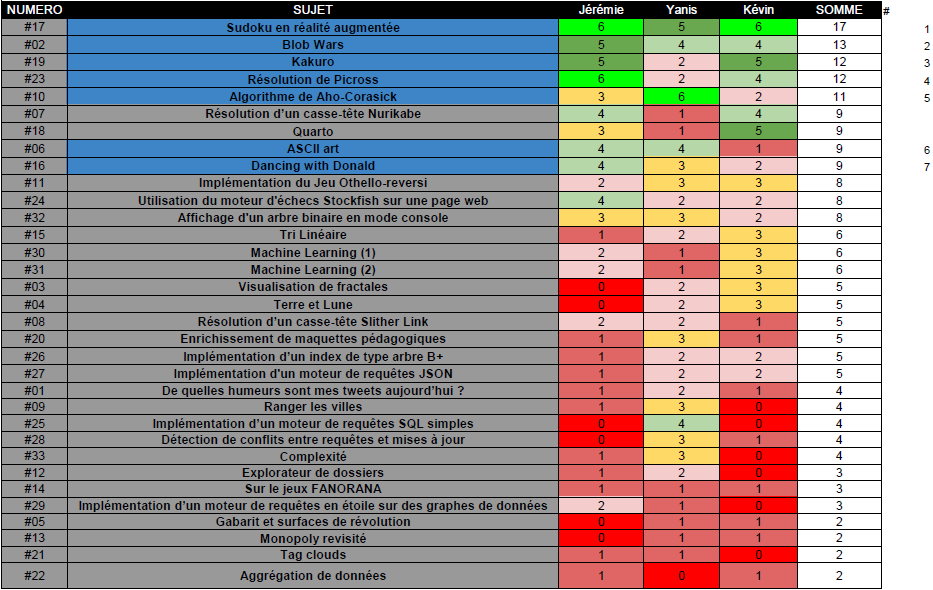
\includegraphics[scale=0.47]{figures/tableur_choix}
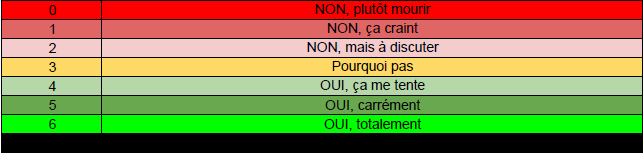
\includegraphics[scale=0.5]{figures/legende_tableur.png}
\caption{Tableur regroupant nos choix de sujets parmi ceux proposés}
\label{fig:Screenshot2}
\end{center}
\end{figure}

Heureusement, c'est là que Jérémie a eu la bonne idée de se servir d'un tableur qu'il a conçu pour l'occasion (Figure \ref{fig:Screenshot2}). Cela a permis de rationaliser le choix des sujets et de leur hiérarchie. Plus important encore, vous observerez que le sujet Blob Wars était notre second choix après le sujet de résolution de sudoku en réalité augmentée mais qu'il était en moyenne apprécié par tout le monde. Jérémie nous a aussi montré qu'il avait la capacité à diriger et superviser un groupe (par exemple en s'occupant de faire les démarches de création de groupe, etc.). Il a donc été naturel qu'il soit le représentant du groupe.\\

Arrivés à la fin du mois de décembre et une fois le sujet attribué, nous avons pris contact une première fois par mail avec M. Bessy et avons convenus d'un premier rendez-vous le 18 janvier 2019. Nous avons gardé un rythme d'une réunion toutes les deux semaines ce qui nous permet d'avancer convenablement et de ne pas rentrer en conflit avec notre cursus universitaire.

\newpage
\section{Diagrammes de classes}

\subsection{\textit{IA}}
\vspace{40px}

\begin{center}
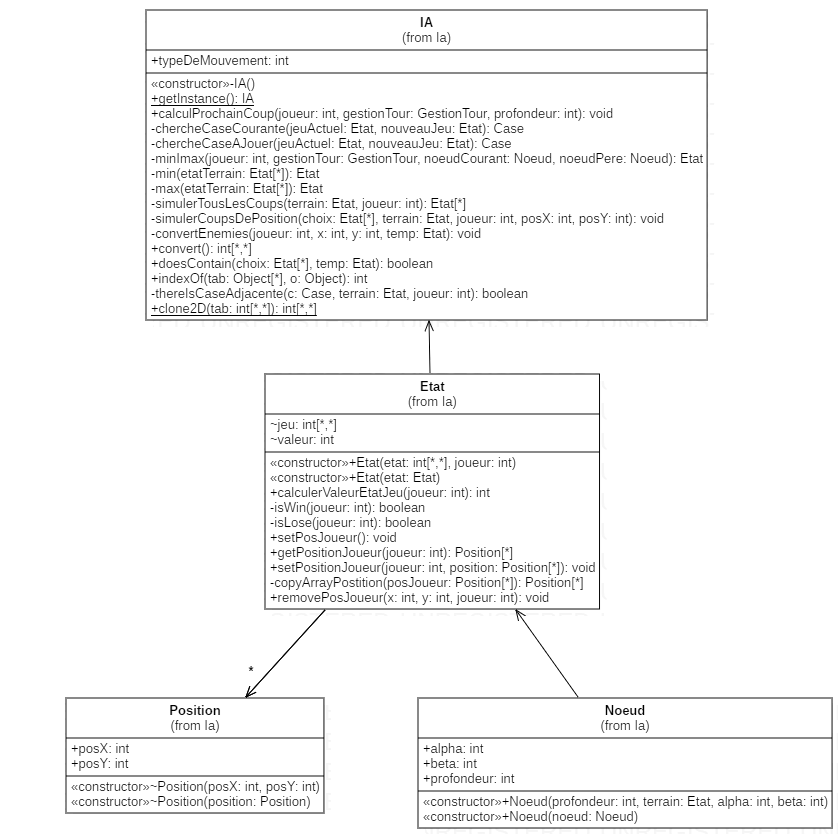
\includegraphics[width=1\textwidth]{UML/IA.png}
\end{center}

\newpage
\subsection{\textit{Engine}}
\vspace{40px}

\begin{center}
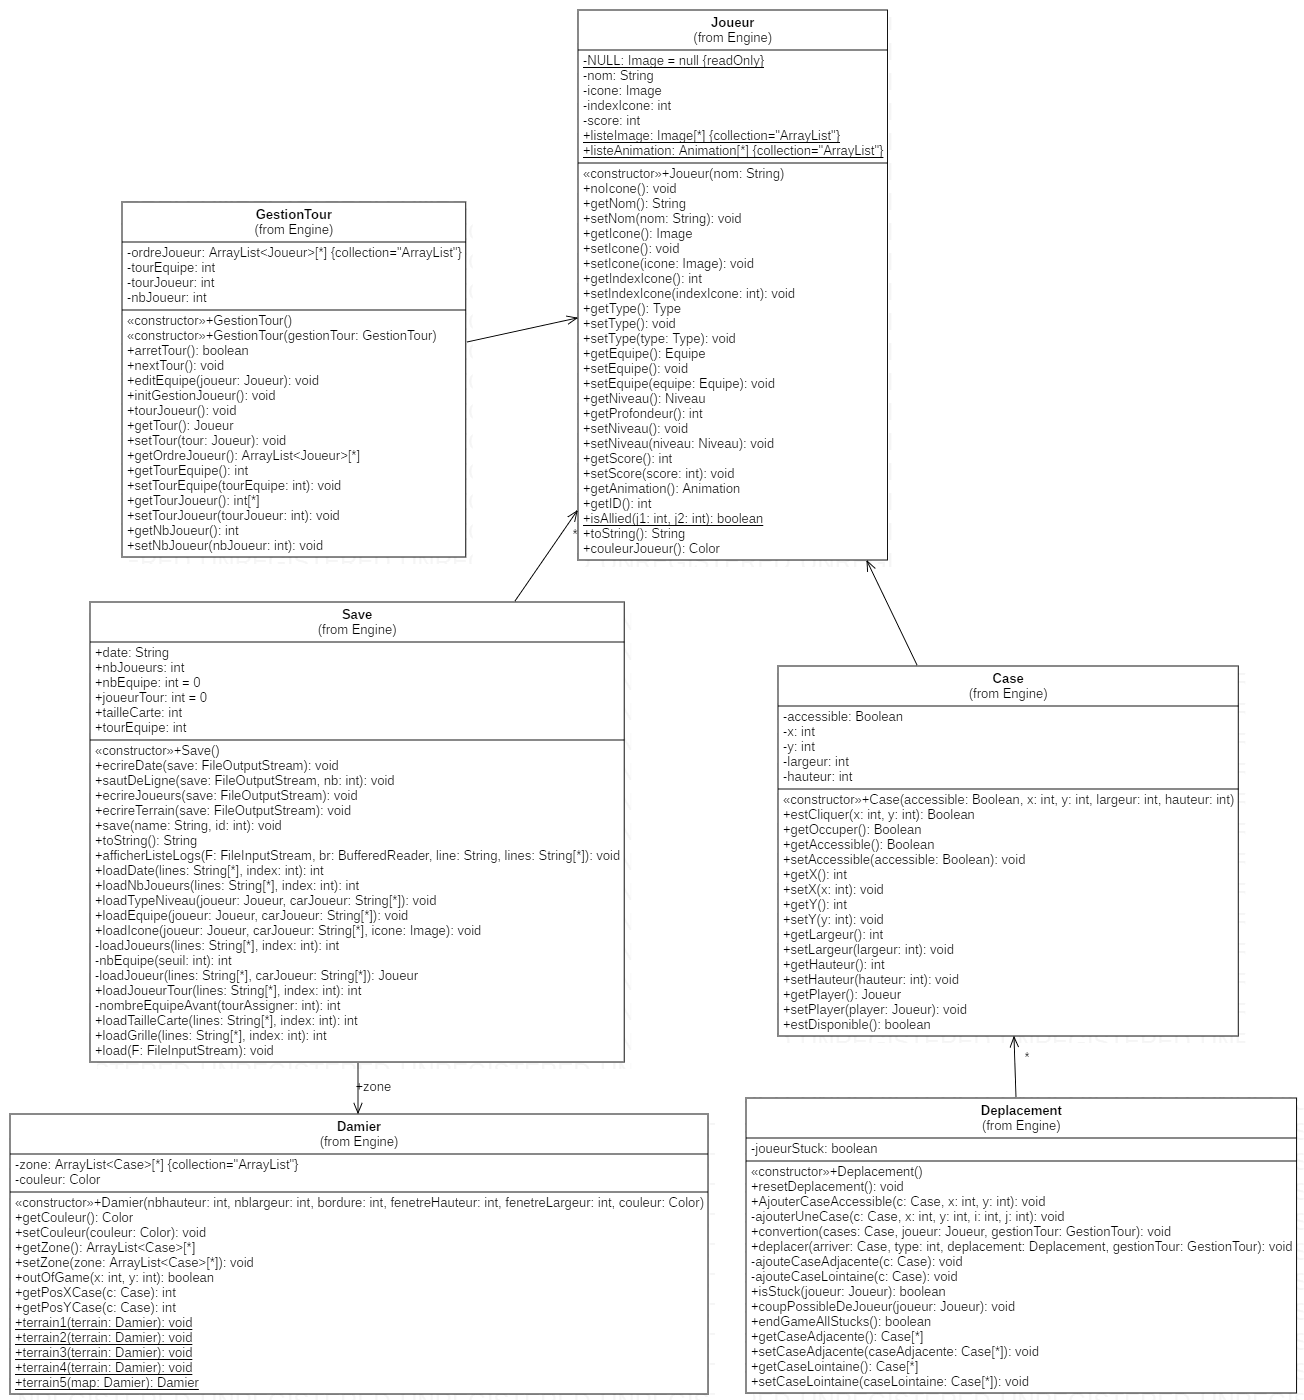
\includegraphics[width=1\textwidth]{UML/engine.png}
\end{center}

\newpage
\subsection{\textit{State}}
\vspace{40px}

\begin{center}
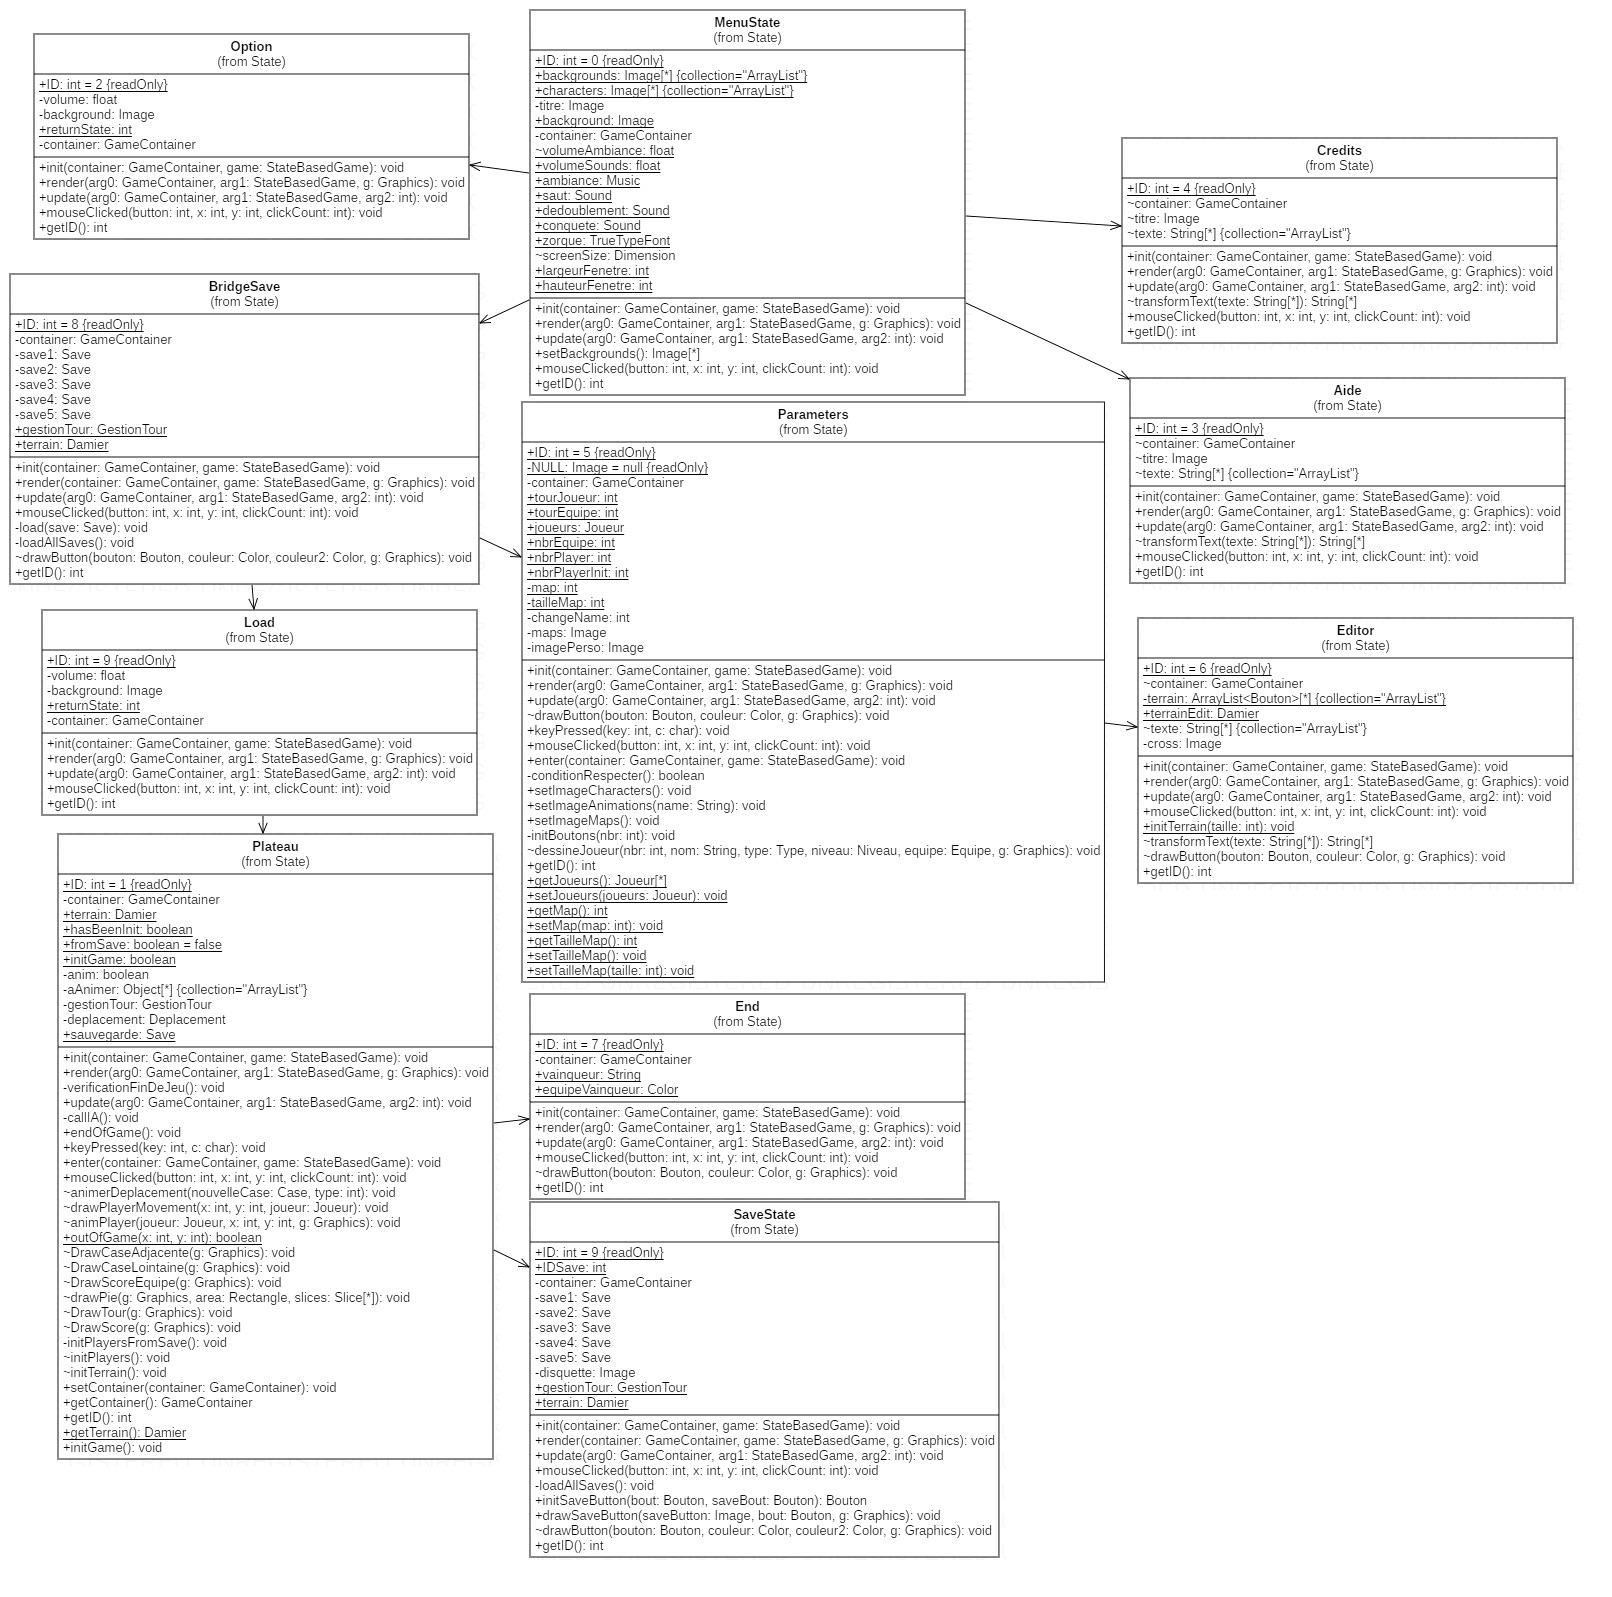
\includegraphics[width=1\textwidth]{UML/state.jpg}
\end{center}

\newpage
\section{Calculs de temps d'exécution de l'algorithme MinMax}

\begin{center}
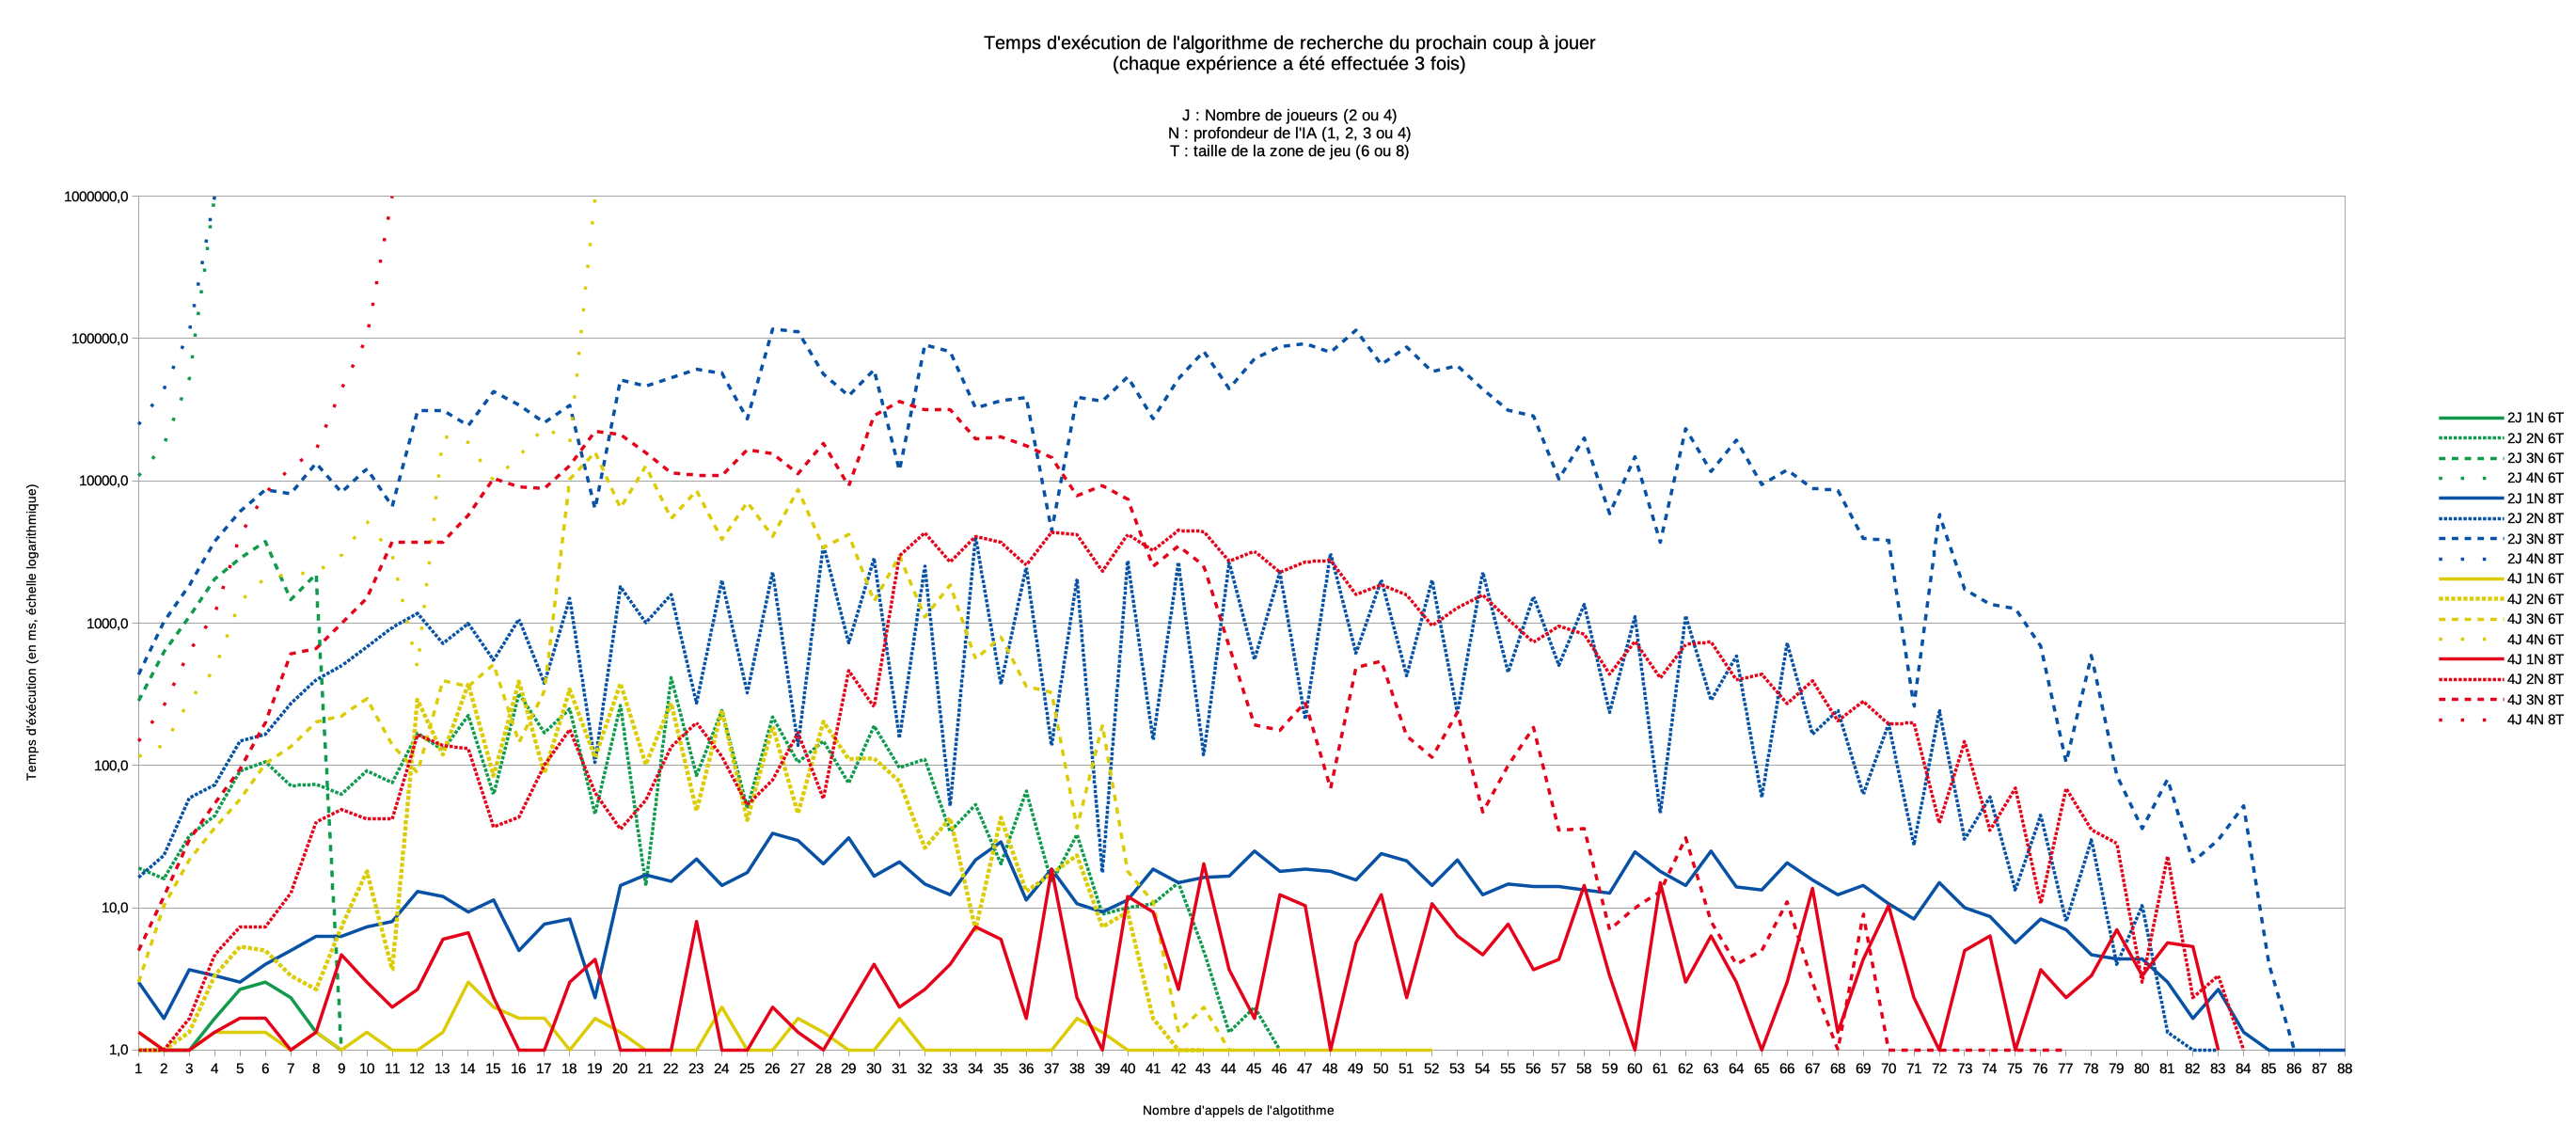
\includegraphics[angle=270,origin=c,scale=0.4]{figures/minmax/Temps_Execution.png}
\label{fig:minMaxTempsExecution}
\end{center}


\newpage
\section{Cahier des charges}

\subsection{Premier RDV}

\begin{itemize}
    \item UML
    \item Gantt
    \item Répartition des tâches
    \item Rapport
\end{itemize}

\subsection{Deuxième RDV}

\begin{itemize}
    \item Code minimal défini dans l'UML
    \item Prototype de jeu fonctionnel
    \item Save
    \item Rapport
\end{itemize}

\subsection{Troisième RDV}

\begin{itemize}
    \item Implémentation Minimax
    \item Implémentation Alpha-Bêta
    \item Load
    \item Rapport
\end{itemize}

\newpage
\section{Rapports d'entrevue}

\subsection{18 Janvier 2019}
Allouch Yanis, Roux Jérémie, Villaroya Kévin et Bessy Stéphane (11 h 08 - 11 h 57)\\

\begin{itemize}[itemsep=5pt]

\item Quid du langage le plus adapté ? Deux choix principaux avec C++ et Java avec respectivement les librairies SFML et Slick.

\item Rappel du fonctionnement du jour de la soutenance orale avec un jury, et une soutenance publique.

\item Stéphane Bessy (notre professeur référent pour ce projet) est spécialisé dans l'algorithmie et les maths.

\item Rendu attendu\footnote{Moodle de l'UE HLIN405 : https://moodle.umontpellier.fr/course/view.php?id=1295} : une archive + un mémoire 10 pages suivant un plan ou d'après Stéphane Bessy : interface graphique qu'est ce qui a été fait ? Diagramme des classes ?...)

\item Première explication des types d'IA possibles : 

\begin{description}
    \item[Niveau 1 :] Simuler toutes les possibilités et maximiser un critère ou des critères (avec une note/point ...) et jouer le meilleur coup de manière locale.
    \item[Niveau 2 :] Faire le niveau 1 mais re-simuler pour l'adversaire avec cette configuration (algo du min/max) et re-simuler avec cette nouvelle configuration le meilleur coup à jouer. On peut étendre cela autant que possible. Point négatif : temps de calcul très grand (Ordre de grandeur/Corrélation entre temps de calcul et la profondeur de décision ?)
\end{description}
 
\item Une version jouable à 2 joueurs est cependant attendue rapidement peu importe que le côté graphique soit pris en charge.
 
\item Cependant, un cahier des charges minimal (pas trop ambitieux) est nécessaire et demandé sous une à deux semaines (nous nous sommes mis d'accord pour le prochain rendez-vous encore non défini au moment de l'entrevue). Ce cahier des charges doit contenir le minimum comme : la version jouable du jeu à 2 au moins, les implémentions qu'on peut d'ores et déjà faire, etc.

\item Récapitulatif des attentes de la prochaine rencontre (nous pourrons commencer à coder seulement après avoir effectué ces tâches) :

\begin{itemize} [label=$\Rightarrow$]
    \item Commencer le rapport (c'est à dire ce qu'on est en train de faire)
    \item Le cahier des charges
    \item Réfléchir à une structure du code
    \item Définir les tâches à réaliser avec un planning (diagramme de Gantt\footnote{Page Wikipédia du diagramme de Gantt : https://fr.wikipedia.org/wiki/Diagramme\_de\_Gantt} avec EdrawMax)
    \item Se répartir les tâches (diagramme en camembert ou directement intégré dans le diagramme de Gantt)
\end{itemize}
 
\end{itemize}

\newpage
\subsection{31 Janvier 2019}
Allouch Yanis, Roux Jérémie, Villaroya Kévin et Bessy Stéphane (14 H 00 - 15 H 04)\\

Les points abordés :
\begin{description}
    
    \item[Une aide] Comme l'IA est difficile à contrer\footnote{Même la plus simple étant donnée qu'elle fait constamment des choix logiques}, proposer une aide qui affiche le 'meilleur' coup potentiel que le bot aurait pu jouer.
    
    \item[Présentation] :
        \begin{itemize}
            \item du diagramme de Gantt.
            \item du diagramme de classe en UML.
            \item du code et d'un prototype qui permet à ce jour :
            \begin{description}
                \item[Joueur] Une sélection\footnote{C'est à dire entre un Pseudo/Image/Equipe} et sa personnalisation pour les 4 joueurs.
                \item[Map Selector] Le choix parmi X plateaux de jeu déjà existants.
                \item[Map Creator] La possibilité de créer sa propre map\footnote{Par ailleurs il est bon de noter qu'une map devra garder une symétrie.}.  
                \item[Volume] L'intégration d'un fond sonore (réalisé par Jérémie) avec volume+\footnote{Réglable par une barre coulissante qui n'est rien d'autre qu'un objet de la Classe \textit{Bouton}} et volume-.
                \item[State] traduit littéralement par un 'état' de jeu qui sont les différentes fenêtres/boutons/états du jeu c'est à dire Menu, Jouer, Credits, Aide, Option, ...
            \end{description}
            \item une mise en ligne du jeu éventuelle via Unity qui permet avec des plugins de gérer du Java ...
        \end{itemize}
        
    \item[Sauvegarde()] Prévoir un moyen de sauvegarder une partie en cours, via une \textbf{"fonction"} d'encodage.
        
    \item[Eval()] Récupérer la fonction d'évaluation de l'IA du site 1980-games\footnote{http://www.1980-games.com/} en faisant du reverse engineering\footnote{La rétro-ingénierie, ou ingénierie inverse ou inversée, est l'activité qui consiste à étudier un objet pour en déterminer un.} et d'un autre côté aller à tâtons pour la notre et l'optimiser au maximum.
    
    \item[IA] \begin{itemize}
        \item Implémenter le Minimax
            \begin{itemize}[label=\textbullet]
                \item On maximise la prise de position sur les bords plus orientée défensive puis offensive
            \end{itemize}
        \item Implémenter Alpha-Bêta
    \end{itemize}
\end{description}

\newpage
\subsection{14 Février 2019}
Allouch Yanis, Roux Jérémie, Villaroya Kévin et Bessy Stéphane (14 H 00 - 14 H 31)\\

Les points abordés :
\begin{enumerate}
    \item Revoir les règles du jeu (correction + ajout pour le PAT par exemple)
    \item Fonction "d'échec et mat" : le "PAT" est buggé mais si le terrain connexe normalement il a une case qui touche le jour à chaque fois ?....
    \item Explication de la structure sous-jacente au jeu: plateau de jeu, case, joueur ...
    \item Une boucle de -1 à 1 pour avoir les cases jouables en gris foncé
    \item La même boucle appliquée "depuis" la première pour avoir les autres cases jouables en un gris clair\footnote{la couleur permet de différencier le type de déplacement effectué}
    \item Animation à revoir
    \item Faire la fonction Eval() pour intégrer une IA
    \item Inclure un diagramme pour représenter le score et se passer du bug de l'encadré gris pour les joueurs
    \item Pouvoir activer une aide 
    \item La fonction Save() "d'encodage"
    \item Ça ne vaut pas le coup de garder l'arbre calculé pour chaque nouveau tour car possiblement le temps de calcul pour parcourir l'arbre sera supérieur à le re-calculer ...
    \item Pouvoir "simuler" une partie
    
\end{enumerate}
\begin{tabular}{c}
    \hline
\end{tabular}
\\
Ce début de réunion a débuté sur une remarque de M. Bessy sur les règles écrites pour notre jeu qui ne sont pas très claires pour une personne qui ne connaît pas le jeu.\\
En effet des étourderies de français, franglais présentes ont dûes être corrigées. Ensuite une imprécision sur la façon de jouer a été corrigée (sur les cases "adjacentes" à deux de là où il se trouve, le pion sera déplacé.). Au final nous avons ré-écrit les règles en changeant le mot "blob" par "pion" en incluant la notion de couleur dans les déplacements qui permet au joueur de manière intuitive de comprendre qu'il existe une différence dans le choix des cases que lesquelles se déplacer ou se dupliquer.\\
On a aussi mentionné le fait qu'on a inclut une fonction qui permet de faire un PAT\footnote{Référence au pat des échecs, qui apparaît quand on veut faire une égalitée avec son adversaire} cependant elle a besoin de quelques ajustements.\\
Le troisième point ayant \textbf{une importance pour M. Bessy} qui souhaite voir apparaître une explication détaillée de structures sous-jacentes aux fonctionnement du jeu, des choix effectués, etc. Par exemple comment les positions sont calculées.\\
Pour le cinquième point c'est un détail esthétique qui est loin d'être prioritaire, cependant, pour un produit final, il serait en effet bon de revoir les effets de transition et de garder un jeu assez fluide. Dans le même genre, on a la représentation du score qu'on peut dire classique jusqu'à maintenant qui pourrait éventuellement changer pour une représentation en camembert ou autre diagramme plus visuel et moins "buggé".\\
D'un autre coté \textit{la fonction d'évaluation} pour juger quel déplacement est plus intéressant qu'un autre n'est toujours pas codée/fonctionnelle, ce qui nous empêche d'implémenter le \textit{Minimax}.
Par ailleurs ça influe aussi sur l'ajout d'une fonction d'aide pour le joueur humain étant donné l'absence d'une IA.\\
Sinon sans avoir pour le moment codé le nécessaire, M. Bessy nous a apporté une réponse à une question qu'on se posaient pour optimiser les calculs sur les coups à jouer représentés avec un arbre\footnote{pour le moment d'une hauteur maximale théorique 3} : "le temps de calcul de parcours de l'arbre sera peut-être plus long/important que le calcul de l'arbre lui-même". Donc nous n'allons pas nous compliquer la tâche mais concevoir une IA implémentée de manière brute.\\
A la suite de ça, nous pourrons alors d'après notre conception du jeu permettre une "simulation"\footnote{expressément demandée par M. Bessy} de partie entre deux IA.\\
Finalement le dernier point abordé est la fonction de sauvegarde pour immédiatement fixer un format de sauvegarde.


\newpage
\subsection{28 Février 2019}
Allouch Yanis, Roux Jérémie, Villaroya Kévin et Bessy Stéphane (14 H 12 - 15 H 00)\\

Les points abordés :
\begin{enumerate}
    \item La fin de partie "PAT" précédemment buggée a été légèrement modifiée et prend en charge les fins de parties en 1v1\footnote{peu importe le nombre de joueurs c'est le nombre d'équipe/couleur qui importe car c'est une boucle qui itère sur ces derniers qui permet de faire appel à endOfGame() }
    \item Système de sauvegarde
    \item Fonction/Méthode d'évaluation du terrain (this.calculerScoreTerrain() )
    \item Structure sous-jacente, peu de choses à dire
    \item On arrive doucement à un produit opérationnel
    \item Une collection de Collection x Collection pour les coups possibles
    \item Load() Charger une partie
    \item Débugger le PAT pour N équipes
    \item Finir l'implémentation de l'IA : Minimax() > Min(), Max()
    \item Du scripting pour faire des stats ...
    \item Yanis : Debug le PAT()
    \item Jérémie : Implémente le load()
    \item Kévin : Finit d'implémenter le Minimax()
\end{enumerate}

\begin{tabular}{c}
    \hline
\end{tabular}
\\
    Réunion assez sommaire avant ce début de vacances, il n'y a pas eu d'avancées majeures dans le jeu. \\ 
    La plupart du temps étant alloué à l'IA, d'un autre côté nous n'avons pas de structure sous-jacente à présenter à M. Bessy plus détaillée que ce qu'on lui avait déjà fournit. \\
    Nous avons défini ensemble l'objectif de la prochaine réunion qui est d'avoir un jeu 100\% opérationnel dans tous les cas dans un premier temps ce qui inclut une sauvegarde de parties et la reprise de celle-ci.\\
    Il faut que le jeu se termine correctement avec plusieurs équipes en jeu et finalement avoir une IA qui fonctionne. \\
    
    La prochaine réunion est fixée au 18 mars 2019.

\newpage
\subsection{18 Mars 2019}
Allouch Yanis, Roux Jérémie, Villaroya Kévin et Bessy Stéphane (13 H 53 - 14 H 42)\\

Les points abordés :
\begin{enumerate}
    \item IA 
    \begin{itemize}
        \item Algorithme Minmax implémenté
        \item Optimiser le calcul de coup (heuristique)
        \item La taille du plateau de jeu impacte le temps de calcul de chaque coup
        \item IA du site TwoPlayersGames.org
    \end{itemize}
    \item Fonction de sauvegarde terminée
    \item Fonction de chargement présente des bogues
    \item Détail de la fonction d'évaluation
    \item Remarque sur le rapport
    \item Remarque sur l'algo Minmax
    \label{entrevue:18mars}
\end{enumerate}

\begin{tabular}{c}
    \hline
\end{tabular}\\

    Lors de cette réunion après 3 semaines (avec 1 semaine de vacance) pour avancer le projet, nous avons fait une petite démonstration IA vs IA avec différentes profondeurs. \\
    S'en suit une explication de la fonction d'évaluation telle que décrite ci-après. La fonction d'évaluation attribue un point à chacun des pions sur le plateau et plus un coup possible permet de créer de pions, plus il est \textbf{intéressant}. \\ 
    Ce qui a mis en évidence ce que vous avions déjà remarqué lors de nos phases de test, d'abord le temps de calcul est fortement impacté par la taille du plateau et qu'il faudra qu'on optimise la façon dont les coups sont calculés (c'est aà dire ne sauvegarder que les coups "jouables" et non pas un \textbf{ArrayList} < des plateaux possibles > représentés tels quels \textbf{ArrayList}< \textbf{ArrayList} < de position/case > >).\\
    Par ailleurs, après une première étude du code source\footnote{Voir https://pastebin.com/8gFy3qPH}, on tire la conclusion que leur IA n'est basée que sur du backtracking\footnote{étant donnée la structure du code} avec une fonction d'évaluation qui est diluée dedans (ce qui ne la rend pas explicite et compréhensible). Donc nous laissons cette éventualité de côté pour le moment.\\
    Plus encore, lors de cette réunion Jérémie a pu terminé la fonction save qui ne présente plus de bug qui aurait pu être rapportée lors de la précédente réunion cependant certains bugs persistent dans la fonction de chargement.\\
    Kévin a fait une remarque très pertinente sur l'écriture du code d'une méthode qui ne devrait pas prendre plus d'une dizaine de ligne qui rendu possible par une imbrication de méthode qui procède à des test unitaires.\\
    L'avant dernier point étant une remarque pertinente sur le rapport mais tout à fait normale étant donné que le développement du plan n'a pas encore vraiment débuté et mise à part les quelques fautes d'orthographes alors présentes dans ce dernier.\\
    Il faudra au moins une partie où nous justifirons le choix du langage, de la librairie et une autre qui explique en terme algorithmique le Minmax avec une analyse de complexité si nécessaire.\\
    Pour terminer cette réunion, M. Bessy à fait une précision quand à l'optimisation de notre algorithme en supprimant la ligne 103 dans la classe IA qui implique de calculer chaque noeud découvert\footnote{et dont la valeur sera au final écrasée par celle venant des feuilles} alors que l'algorithme veut qu'on calcule à partir des feuilles.\\
    
    La prochaine réunion est fixée au 27 mars 2019, finalement reportée au 02 avril 2019.


\newpage
\subsection{02 Avril 2019}
Allouch Yanis, Roux Jérémie, Villaroya Kévin et Bessy Stéphane (15 H 30 - 16 H 17)\\

Les points abordés :
\begin{enumerate}
    \item Remarque sur le rapport
    \item IA
    \begin{itemize}
        \item Minimax
        \item Alpha-Bêta
        \item Amélioration, granularité
        \item Fonction d'évaluation
    \end{itemize}
    \item Fin du jeu
    \item Fonction de chargement
    \item Interface WEB
    \item Complexité
    \item Une conclusion + explication d'une soutenance
\end{enumerate}

\begin{tabular}{c}
    \hline
\end{tabular}\\
    
    Il faut noter que nous avions choisi de reporter cette réunion d'une semaine par rapport à la date prévue, c'est à dire au 2 avril pour avoir plus de matière à travailler avec M. Bessy.\\
    
    Pour le premier point, une remarque de M. Bessy qui a trouvé notre rapport plutôt correct. Il y a cependant plusieurs points à améliorer comme une meilleure explication de l'implémentation de l'IA et d'une analyse de complexité du Minimax ou encore une conclusion à rajouter. Kévin suggère de supprimer la partie "ANNO 2018" qui pour le moment explique brièvement comment le groupe s'est formé (avec une touche d'humour ?) qui selon lui ne fait pas de sens. Jérémie est intervenu à ce sujet et pense au même titre que Yanis qu'il faudrait revoir aussi ce paragraphe et nous sommes d'accord pour revoir la section Introduction.\\
    
    Ensuite, le second point le plus important de la séance qui est la raison principale du report de la réunion est l'implémentation du Minimax qui a été améliorée et débuggée par Kévin en tenant compte des précisions sur le code par M. Bessy lors de la précédente réunion qui fait le bon calcul cette fois-ci. Il suggère aussi l'ajout d'un random dans le choix du meilleur coup a jouer\footnote{Lors de plusieurs choix possibles}\footnote{On distingue un vrai changement "comportemental" dans la façon de jouer de l'IA qui est moins bête} et une première tentative d'implémentation de l'Alpha-Bêta qui à ce jour n'est pas complète. Une remarque de Kévin est qu'il ne comprend pas pourquoi cet algorithme arrive à faire remonter l'alpha et le bêta d'un autre coup et qui pense que ça vient de là.\\
    
    Pour déboguer la fin du jeu, on repart sur une base propre. Le code associé à la fin du jeu\footnote{endOfGame et endOfGameAllStuck et la méthode isStuck} a été supprimé pour repartir sur une bonne base au lieu d'essayer de comprendre ce qui avait été écrit.\\
    
    La fonction de chargement d'une partie\footnote{Une unique partie à ce jour}. Nous avons pour idée d'implémenter une interface qui permet de charger 5 sauvegardes au maximum\footnote{De manière arbitraire}. L'interface de re-jouabilité serait accessible depuis la slide Jouer avec un bouton "Charger" pour ne pas changer des \textbf{design patterns de conception} usuels.\\
    
    S'en suit une explication courte de l'évaluation de la soutenance qui se compose de 15 min de prestation orale avec un premier plan possible :
    \begin{itemize}
        \item Commencer par une démonstration
        \item Suivi d'une mise en perspective pour expliquer comment on a fait ? (pour que tout prenne son sens)
        \item Expliquer deux ou trois problèmes avec le support projeté\footnote{Des diapositives}
    \end{itemize}
    
    Pour la prochaine fois on aura au moins fait l'élagage du Minimax et réparé de bug de la fin du jeu.\\
    
    La prochaine réunion est fixée au 11 avril 2019.

\newpage
\subsection{11 Avril 2019}
Allouch Yanis, Roux Jérémie, Villaroya Kévin et Bessy Stéphane (11 H 51 - 12 H 41)\\

Les points abordés :
\begin{enumerate}
    \item Observation temps de calcul coup/ia/nbJoueur/prof/tailleTab
    \item Analyse Alpha-Beta
    \item Seconde observation du temps de calcul sans elagage
    \item Faire un bot
    \item L'interface de re-jouabilité
    \item Peaufinage des graphismes
    \item Pat
    \item Monitoring
    \item Ré-explication du déroulé de la soutenance
\end{enumerate}

\begin{tabular}{c}
    \hline
\end{tabular}\\
    
    Lors de cette réunion, Jérémie avait proposé de se concentrer sur une analyse avec comme objectif l'étude du temps de calcul de chaque coup sur une partie complète par IA pour voir à quel niveau on pouvait se limiter par exemple. Avec comme paramètre d'étude la profondeur d'une IA, le nombre d'IA en partie, et la taille d'un plateau de jeu.\\
    Il sera fait pour la prochaine fois éventuellement une analyse sans l'élagage pour avoir plus de matière à comparer.
    Les dents de scie sont présentes sur le graphique actuel car les mesures ont été faites telles qu'elles : on fait un cumul du temps nécessaire aux mêmes IA pour un coup donné.\\
    On précise un peu plus la fonction d'évaluation, si on arrive à finir complètement l'adversaire\footnote{On rappelle qu'un adversaire ce sont tous les autres pions qui ne sont pas de notre équipe} on compte 100 points\footnote{On rappelle que de base un "blob" de plus donne 1 point en plus} de plus. \\
    Au cours de la réunion, M. Bessy a ramené une idée très intéressante par rapport au jeu déjà existant : faire jouer notre IA contre celle du jeu en ligne\footnote{La version flash qu'on avait reverse} pour voir laquelle est la plus \textbf{forte}.\\
    Pendant cet échange, Yanis a proposé de faire un bot codé en AutoIT par exemple, mais n'importe quelque langage de scripting\footnote{Exemple LUA, Python} pourrait tout aussi fonctionner. AutoIT a simplement une bonne réputation pour ce qui est de faire des macros, des mini-bots mouse-clicker.\\
    Comme idée de développement future, on peut changer les animations (en l'état comment les animations sont codées il suffit de changer les sprites)\footnote{ressources des animations, les images de base} et quelques lignes de code pour que ce soit effectif.\\
    Mais aussi proposer à l'utilisateur de changer le BG\footnote{Background}, l'UI\footnote{User-Interface} pour que ça devienne au goût de tout le monde.\\
    Le PAT a été complètement re-codé, malheureusement même si les fins de jeu sont opérationnelles, parfois des PAT arrivent alors qu'il n'y a pas de raison.
    Par exemple J1 peux encore jouer mais J2 non et malgré que ce soit au tour de J1, il y a PAT.\\
    Pour rester dans les idées à venir à programmer, il y a un fichier de log qui aurait pour objectif de monitorer plus facilement les parties avec une granularité très fine\footnote{Timestamps à chaque coup + la case joué de où à où} pour pouvoir faire par exemple des statistiques aisément.\\
    Il faudra cependant voir comment gérer les I/O pour que cela reste performant.\\
    On a par ailleurs toujours ce \textbf{doute} que l'alpha-bêta ne calcule pas ce qu'il calcule et M. Bessy aimerait bien qu'on enlève ce doute pour la prochaine réunion et la fin du projet.\\
    

    La prochaine réunion est fixée au 26 avril 2019.
    
    
\newpage

\subsection{26 Avril 2019}
Allouch Yanis, Roux Jérémie, Villaroya Kévin et Bessy Stéphane (09 H 45 - 10 H 20)\\

Les points abordés :
\begin{enumerate}
    \item Rapport de TER
\end{enumerate}

\begin{tabular}{c}
    \hline
\end{tabular}\\
    
    Cette réunion s'est déroulée assez rapidement. L'examen approchant, peu d'évolutions significatives au niveau code par rapport au mémoire.\\
    
    Par ailleurs, M.Bessy a très fortement insisté pour avoir un rapport final lors de la prochaine réunion. Celui-ci devrait contenir une conclusion sur 3 points avec : un bilan de ce qui a été fait et ce qu'on en retire, un bilan des compétences utilisées, des perspectives d'avenirs. La réunion s'est terminé sur cela.\\
    
    La prochaine réunion est fixée au 7 mai 2019.

    
\newpage

\subsection{7 mai 2019}
Allouch Yanis, Roux Jérémie, Villaroya Kévin et Bessy Stéphane (16 H 14 - 16 H 35)\\

Les points abordés :
\begin{enumerate}
    \item Rapport de TER.
    \item Soutenance orale.
\end{enumerate}

\begin{tabular}{c}
    \hline
\end{tabular}\\
    
    À la différence de la précédente réunion, une avancée dans le code a été faite, l'élagage fonctionne enfin, tout du moins les temps de calculs sont devenus corrects tel que attendu. En effet, on peut maintenant jouer avec une profondeur 5 voire 6 sans faire planter le jeu en 2v2 par exemple étant donnée qu'on est passé d'une minute de calcul à quelques secondes.\\
    
    Pour ce qui est du rapport, M. Bessy est très content de la qualité de celui-ci. Miss à part quelques étourderies (se reporter au rapport imprimé corrigé par M. Bessy) qui seront corrigées pour la version déposée sur le Moodle.
    
    Pendant la réunion, Jérémie a fait savoir qu'on avait reçu notre date de soutenance orale qui est fixée au 21 mai 2018\footnote{Lien vers le document http://tiny.cc/BlobWarsAnnexe1} à 16h30 en 16.50. Notre jury sera composé de :
    \begin{itemize}
        \item Anne-Muriel Chifolleau
        \item Philippe Jansen
        \item Federico Ulliana
    \end{itemize}
    
    La prochaine réunion sera dédiée à une répétition de la soutenance orale. Cette réunion est fixée au 20 mai.

    
\newpage

\section{Rapports de version}

\definecolor{rouge}{RGB}{255,0,0}
\definecolor{vert}{RGB}{0,128,0}

\subsection{Légende}
% Non Résolu
%
\begin{itemize}[label=\CheckmarkBold, font=\color{rouge}]
    \item Exemple de description d'un bogue non résolu
\end{itemize}

% Résolu
%
\begin{itemize}[label=\CheckmarkBold, font=\color{vert}]
    \item Exemple de description d'un bogue résolu
\end{itemize}
% Suggestion non réalisé
%
\begin{itemize}[label=\Peace, font=\large \color{rouge}]
    \item Exemple de description d'une suggestion non implémentée
\end{itemize}
% Suggestion réalisée
%
\begin{itemize}[label=\Peace, font=\large \color{vert}]
    \item Exemple de description d'une suggestion implémentée
\end{itemize}

%%%%%%%%%%%%%%%%%%%%%%%%%%%%%%%%%%%%%%%%%%%%%%%%%%%%%%%%%
%%%%%%%%%%%%%%%%%%%%%%%%%%%%%%%%%%%%%%%%%%%%%%%%%%%%%%%%%

\subsection{2 Février 2019 (V1)}
% Bogues pas résolu
%
\begin{itemize}[label=\XSolidBrush, font=\color{rouge}]
    \item Fin de partie quand 1 - nombre total de joueur ne peut plus jouer (mais dont il reste au moins une case)
    \item Fin de partie quand toutes les cases sont occupées
\end{itemize}
% Suggestions
%
\begin{itemize}[label=\Peace, font=\large \color{rouge}]
    \item Ajouter le score en étiquette du diagramme en camembert
    \item Indiquer les joueurs avec le nom en couleur et l'icône de leur personnage si possible en les séparant par équipe (le tout sous forme d'un tableau/liste)
    \item Switch On-Off les animations
    \item Un bouton dans 'HOME' qui configure et lance $x$ parties automatiquement et permettent de sauvegarder le résultat
    \item Un Timer pour avoir des données plus précises.
    \item Threads
\end{itemize}

%%%%%%%%%%%%%%%%%%%%%%%%%%%%%%%%%%%%%%%%%%%%%%%%%%%%%%%%%
%%%%%%%%%%%%%%%%%%%%%%%%%%%%%%%%%%%%%%%%%%%%%%%%%%%%%%%%%

\subsection{17 mars 2019 (V2)}

%Bugs non resolu
%
\begin{itemize}[label=\CheckmarkBold, font=\color{rouge}]

\end{itemize}
% Bogues résolu
%
\begin{itemize}[label=\CheckmarkBold, font=\color{vert}]
    \item Cadres des équipes et de l'annonce du tour qui empiètent sur le terrain
    \item Terrain non-régénéré lors du lancement d'une nouvelle partie sans relancer l'application
    \item Accents qui disparaissent (lors du passage par Git Windows ?)
    \item Blanc lors du "bouclage" de la musique (blanc à la fin du fichier audio)
    \item Considère qu'une case adjacente à deux ne peut être atteinte que lorsqu'au moins une case directement adjacent peut être atteinte
    \item Lorsqu'on sélectionne un terrain personnalisé et des listes de personnages et si on clique sur Confirmer, alors, affichage d'un fenêtre avec "PAT".
\end{itemize}
% Suggestions
%
\begin{itemize}[label=\Peace, font=\large \color{vert}]
      \item Diagramme en camembert qui représente la proportion d'occupation de chaque équipe
\end{itemize}

\subsection{11 avril 2019 (V3)}

%Bugs non resolu
%
\begin{itemize}[label=\CheckmarkBold, font=\color{rouge}]
\end{itemize}
% Bogues résolu
%
\begin{itemize}[label=\CheckmarkBold, font=\color{vert}]
    \item IA vs IA d'un niveau important fait planter le render()
    \item Le load() plante quand une IA est concernée ?
    \item Les fins de parties sont prises en charge, plus de crash quand il y a une IA en jeu
\end{itemize}
% Suggestions
%
\begin{itemize}[label=\Peace, font=\large \color{red}]
    \item Une mise sur le WEB
    \item Revoir les animations
    \item Proposer une personnalisation de l'interface
    \item Un bot pour faire jouer notre version contre une autre
\end{itemize}


\subsection{7 mai 2019 (V4)}

%Bugs resolu
%
\begin{itemize}[label=\CheckmarkBold, font=\color{vert}]
    \item Élagage
    \item PAT    
\end{itemize}
%%%%%%%%%%%%%%%%%%%%%%%%%%%%%%%%%%%%%%%%%%%%%%%%%%%%%%%%%
%%%%%%%%%%%%%%%%%%%%%%%%%%%%%%%%%%%%%%%%%%%%%%%%%%%%%%%%%

\end{document}